% !Mode:: "TeX:UTF-8"

\chapter[基于多模态引导和样本挖掘的少监督域迁移]{基于多模态引导和样本挖掘的少监督域迁移}[]
\chaptermark{基于多模态引导和样本挖掘的少监督域迁移}
% 图表与公式编号按章重置并显示为 "章-序"（X-Y）格式，
% 由 book.cls 的 \newcounter{figure}[chapter] / \@addtoreset{equation}{chapter}
% 与 hithesisbook.cls 的 \thefigure / \thetable 定义共同保证；
% 此处不可再调用 \counterwithin，它会把编号改写为 "X.Y" 且全局泄漏到后续章节。

\section{引言}

上一章围绕无监督模型迁移设定，本章进一步讨论再有限监督下如何提升模型迁移性能。
少监督模型迁移涵盖半监督、少样本与主动等多种设定，其核心挑战在于：如何在极为有限的标注预算下最大化监督信号的信息量。当标注预算极为稀缺时，监督信号的构造面临双重约束：一方面需要在无标注数据中主动挖掘高价值样本，以最小的标注代价换取最大的监督信息增量；另一方面需要借助外部知识源拓展监督信号的覆盖范围与判别可靠性。视觉—语言模型凭借大规模图文对比预训练积累了丰富的开放语义判别能力，其预测不依赖源域分布，能够为稀缺标注场景下的跨域迁移提供与任务驱动监督互补的语义判断信号。然而，如何建立视觉—语言模型与源模型在信息驱动采样与双向深度协同层面的严谨理论框架，仍是一个尚未解决的关键问题。

针对上述挑战，本章围绕稀缺监督条件下的信息最大化问题，沿样本筛选与跨模型协同两个角度协同推进。在样本筛选层面，借助信息驱动的主动采样机制在无标注目标域中挖掘高价值样本，以最小的标注代价换取最大的监督信息增量；在跨模型协同层面，借助视觉—语言模型的开放语义判别能力实现与源模型的双向深度协同，在避免视觉—语言模型丧失泛化能力的同时实现两类监督信号的互补融合。为建立理论指导，本章推导了少监督场景下的协作风险上界，揭示了双假设空间下的样本覆盖、视觉—语言模型的目标域风险与跨模型对齐损失三个关键因素的协同优化目标，为后续模块设计提供可量化的优化目标。实验在闭集与开放集两种设定下均取得当前最优性能，并展示了所提方法在训练效率与额外开销上的工程实用性。

本章工作可归纳为以下三点：
\begin{enumerate}
    \item 少监督场景协作风险上界理论：建立面向稀缺标注条件下的协作风险上界理论分析，明确主动样本选择、视觉—语言模型适应与跨模型对齐三者的协同优化目标。
    \item DAMF 双主动学习框架：首次将视觉—语言模型引入稀缺标注条件下的模型迁移框架，通过双向蒸馏机制实现其与目标模型的有效交互，在闭集与开放集两种设定下均取得当前最优性能，且训练阶段仅引入可忽略的额外参数量（+0.002M）与显存开销（+0.48 GB）。
    \item 实验验证与综合分析：在 Office、Office-Home、VisDA-C 与 miniDomainNet 四个跨域基准的闭集与开放集两种设定下均取得当前最优性能；闭集与开放集场景下的性能提升均高于现有方法，验证了样本筛选与跨模型协同设计的有效性；在部分跨域任务上，所提方法的精度高于依赖源域数据访问的域适应 与主动域适应方法，说明多模态融合在低资源场景下具备补充价值。
\end{enumerate}

\section{基于多模态基础模型引导的主动域适应方法}

\label{sec:chap3_damf}

在无源主动域适应（Source-Free Active Domain Adaptation, SFADA）设定中，源域模型 $\theta_s$ 在带标签的源域数据集 $\mathcal{S}=\{(x_i,y_i)\}_{i=1}^{n_s}\in(\mathcal{X}^{n_s},\mathcal{Y}_s)$ 上预训练得到。给定无标签目标域数据集 $\mathcal{T}=\{x_i'\}_{i=1}^{n_t}\in\mathcal{X}^{n_t}$（含 $C_t$ 个类别），SFADA 的目标是在标注预算 $B$（$B=|\mathcal{T}_q|=\rho|\mathcal{T}|$，$\rho\in(0,1)$）的约束下，通过主动查询策略 $\pi$ 从 $\mathcal{T}$ 中选取子集 $\mathcal{T}_q$ 进行人工标注，最终使目标模型 $\theta_t$（由 $\theta_s$ 初始化）在目标域上的期望风险最小化。借鉴文献~\cite{wang2023mhpl,chu2022denoised}，本章采用单批次一次性查询策略，即所有标注样本 $\mathcal{T}_q$ 在训练开始前一次性选定。源域数据 $\mathcal{S}$ 在适应阶段不可访问。

目标模型对类别 $k$ 的预测概率定义为 $p_T^{(k)}(x)=\theta_t^{(k)}(x)$。本章同时考虑两种设定：（1）闭集设定，$\mathcal{Y}_s=\mathcal{Y}_t$，$C_s=C_t$；（2）开放集设定，$\mathcal{Y}_s\subset\mathcal{Y}_t$，需要在识别 $C_s$ 个已知类别的同时拒绝其余 $|\mathcal{Y}_u|=|\mathcal{Y}_t|-|\mathcal{Y}_s|$ 个未知类别（统一标记为 ``unknown''）。

为利用跨模态先验，本章引入 ViL 模型 $\theta_v$ 作为辅助监督源。设 $\mathbf{I}=\phi(x)$ 为 ViL 图像编码器提取的图像特征，文本嵌入通过类别级可学习 prompt $\{V_k\}_{k=1}^{C}$ 生成，每个 prompt 结构为 $V_k=\{v_1,v_2,\cdots,v_m,c_k\}$，其中 $c_k$ 为类别名称，初始化模板为 ``a photo of a [$c_k$]''。文本嵌入 $\mathbf{w}_k=\mathrm{Enc}_t(V_k)$ 由冻结的文本编码器生成，则 ViL 模型的预测概率为：
\begin{equation}
p_V^{(k)}(x) = \theta_v(x; V_k) = \frac{\exp(\mathrm{sim}(\mathbf{I}, \mathbf{w}_k)/\tau)}{\sum_{i=1}^{C}\exp(\mathrm{sim}(\mathbf{I}, \mathbf{w}_i)/\tau)},
\label{eq:vil_pred}
\end{equation}
其中 $\mathrm{sim}(\cdot,\cdot)$ 为余弦相似度，$\tau$ 为可学习的温度参数。在整个适应过程中，ViL 模型的图像和文本编码器均被冻结，仅优化类别 prompt 以激活其任务感知能力。

% 为便于本章后续对符号的统一引用，本节将涉及的关键符号汇总于表~\ref{tab:chap3_symbols}。

% \begin{table}[!htbp]
%     \bicaption[tab:chap3_symbols]{}{本章关键符号及其定义}{Table}{Key symbols and their definitions}
%     \vspace{0.5em}\centering\wuhao
%     \setlength{\tabcolsep}{8pt}
%     \resizebox{\textwidth}{!}{
%     \begin{tabular}{ll}
%         \toprule
%         符号 & 含义 \\
%         \midrule
%         $\mathcal{S}$ / $\mathcal{T}$ & 源域 / 目标域数据 \\
%         $\mathcal{X}$ / $\mathcal{Z}$ & 样本空间 / ViL 特征空间，其中 $\mathcal{Z}=\{z\mid z=\phi(x),\forall x\in\mathcal{T}\}$ \\
%         $\mathcal{Y}_{s/t}$ / $C_{s/t}$ & 源 / 目标类别空间 / 类别数 \\
%         $n_{s/t}$ & 源 / 目标样本数 \\
%         $x$ / $y$ & 样本 / 标签 \\
%         $P$ / $Q$ & 目标域 / 源域分布 \\
%         $\hat{P}$ / $\hat{Q}$ / $\widetilde{Q}$ & $\mathcal{T}$ / $\mathscr{L}$ / $\mathcal{T}_q$ 的经验分布，其中 $\mathcal{D}_l=\mathcal{S}\cup\mathcal{T}_q$ \\
%         $f_{P/Q}$ & 目标 / 源标注函数 $\mathcal{X}\to\mathcal{Y}$ \\
%         $f'_P$ & ViL 标注函数 $\mathcal{Z}\to\mathcal{Y}$ \\
%         $\theta_{s/t/v}$ & 源模型 / 目标模型 / ViL 模型 \\
%         $\pi$ / $B$ / $\rho$ & 主动采样策略 / 标注预算 / 采样比例（$B=\rho|\mathcal{T}|$） \\
%         $\mathcal{T}_q$ & 主动标注的目标样本子集 \\
%         $\mathcal{H}$ / $\mathcal{G}$ & $k$-Lipschitz / $k_V$-Lipschitz 假设空间 \\
%         $\mathcal{H}_\epsilon$ & 满足 $\mathcal{S}\cup\mathcal{T}_q$ 上 $L(h,f_Q)\le\epsilon$ 的假设子集 \\
%         $\mathfrak{R}_{n_t}(\mathcal{H})$ & $\mathcal{H}$ 上的期望 Rademacher 复杂度 \\
%         $\eta_{\mathcal{G}}$ & 协同假设空间下的理想最大误差 \\
%         $L$ / $\mathcal{L}_{\mathcal{D}}(h,h')$ / $M$ & 对称 $\mu$-Lipschitz 有界损失 / 经验风险 / 损失上界 $0\le L\le M$ \\
%         $d_{\mathcal{U}}$ / $d_X$ / $d_Z$ / $d_Y$ & 距离函数 $d_{\mathcal{U}}:\mathcal{U}\times\mathcal{U}\to\mathbb{R}_{+}$，分别定义于 $\mathcal{U}=\mathcal{X},\mathcal{Z},\mathcal{Y}$ 上 \\
%         $\phi$ & ViL 图像编码器 $\mathcal{X}\to\mathcal{Z}$ \\
%         $\mathbf{I}$ & ViL 图像特征，$\mathbf{I}=\phi(x)$ \\
%         $c_k$ / $V_k$ / $\mathrm{Enc}_t(\cdot)$ / $\mathbf{w}_k$ & 类别 $k$ 的名称 / 可学习 prompt 模板 / ViL 文本编码器 / 文本嵌入 $\mathbf{w}_k=\mathrm{Enc}_t(V_k)$ \\
%         $\tau$ & ViL 模型的可学习温度参数 \\
%         \bottomrule
%     \end{tabular}}
% \end{table}

\subsection{多模型协作风险上界理论}

基于单模型基于差异的主动域适应（DBALDA）~\cite{mathelin2022discrepancy} 理论框架，本节推导了多模型协同 SFADA 的协作风险上界。

设假设空间 $\mathcal{H}$ 由 $k$-Lipschitz 函数组成：$\forall h\in\mathcal{H},\forall x,x'\in\mathcal{X}: d_Y(h(x),h(x'))\leq k\cdot d_X(x,x')$。类似地，ViL 假设空间 $\mathcal{G}$ 由 $k_V$-Lipschitz 函数组成。损失函数 $L:\mathcal{Y}\times\mathcal{Y}\to\mathbb{R}^+$ 对称、$\mu$-Lipschitz、有界（$0\leq L(y,y')\leq M$），且满足三角不等式。ViL 图像编码器 $\phi:\mathcal{X}\to\mathcal{Z}$ 为确定性映射。

引理 3.1（UDA设定下目标风险上界~\cite{mathelin2022discrepancy}）。给定标注集合 $\mathcal{D}_l=\mathcal{S}\cup\mathcal{T}_q$，定义 $\mathcal{H}$ 在 $\mathcal{S}\cup\mathcal{T}$ 上的理想最大误差：
\begin{equation}
\eta_{\mathcal{H}} = \min_{h\in\mathcal{H}}\max_{x\in\mathcal{S}\cup\mathcal{T}}\big[L(h(x), f_Q(x)) + L(h(x), f_P(x))\big].
\label{eq:eta_H}
\end{equation}
则对任意 $\epsilon\geq\eta_{\mathcal{H}}$，$h\in\mathcal{H}_\epsilon$ 及 $\delta>0$，以至少 $1-\delta$ 的概率：
\begin{equation}
L_P(h,f_P) \leq L_{\hat{Q}}(h,f_Q) + \underbrace{2k\mu\frac{1}{n_t}\sum_{x'\in\mathcal{T}}d_X(x',\mathcal{D}_l)}_{\text{覆盖项}} + (2\epsilon+\eta_{\mathcal{H}}) + 2\mu\mathfrak{R}_{n_t}(\mathcal{H}) + \sqrt{\frac{M^2\log(1/\delta)}{2n_t}}.
\label{eq:uda_bound}
\end{equation}

引理 3.2（SFDA设定下目标风险上界）。由于源域数据 $\mathcal{S}$ 不可访问，将式 \eqref{eq:uda_bound} 中的 $\mathcal{L}$ 替换为 $\mathcal{T}_q$，并将理想最大误差限制在目标域 $\mathcal{T}$ 上：
\begin{equation}
\eta'_{\mathcal{H}} = \min_{h\in\mathcal{H}}\max_{x\in\mathcal{T}}\big[L(h(x), f_Q(x)) + L(h(x), f_P(x))\big],
\end{equation}
则以至少 $1-\delta$ 的概率，对任意 $h\in\mathcal{H}'_{\epsilon}$ 及 $\epsilon'\geq\eta'_{\mathcal{H}}$：
\begin{equation}
L_P(h,f_P) \leq L_{\tilde{Q}}(h,f_Q) + 2k\mu\frac{1}{n_t}\sum_{x'\in\mathcal{T}}d_X(x',\mathcal{T}_q) + (2\epsilon'+\eta'_{\mathcal{H}}) + 2\mu\mathfrak{R}_{n_t}(\mathcal{H}) + \sqrt{\frac{M^2\log(1/\delta)}{2n_t}},
\label{eq:sfda_bound}
\end{equation}

引理 3.3（跨空间Lipschitz迁移）\label{cross_lip_trans} 对任意 $x'\in\mathcal{T},x\in\mathcal{T}_q$：
\begin{equation}
\big|L(f_P(x'),f'_P(x')) - L(f_P(x),f'_P(x))\big| \leq \mu\big[kd_X(x',x) + k_Vd_Z(\phi(x'),\phi(x))\big].
\label{eq:cross_lipschitz}
\end{equation}

定理 3.4（协同SFADA风险上界）\label{theorem_coll} 设 $f'_P$ 为 $\mathcal{Z}\to\mathcal{Y}$ 的 ViL 标注函数，定义 $\mathcal{G}$ 关于 $\mathcal{H}$ 在 $\mathcal{T}$ 上的理想最大误差：
\begin{equation}
\eta_{\mathcal{G}} = \min_{g_V\in\mathcal{G}}\max_{x\in\mathcal{T}}\big[L(h(x),g_V(x)) + L(g_V(x),f'_P(x))\big].
\end{equation}
则以至少 $1-\delta$ 的概率：
\begin{align}
L_P(h,f_P) \leq {} & L_{\tilde{Q}}(f_P,f'_P)
 + \underbrace{\mu\frac{1}{n_t}\sum_{x'\in\mathcal{T}}\big[kd_X(x',\mathcal{T}_q) + k_Vd_Z(\phi(x'),\mathcal{T}_q)\big]}_{\text{覆盖项}} \notag\\
& + \eta_{\mathcal{G}} + 2\mu\big[\mathfrak{R}_{n_t}(\mathcal{H}) + \mathfrak{R}_{n_t}(\mathcal{G}\circ\phi)\big]
 + 2\sqrt{\frac{M^2\log(3/\delta)}{2n_t}}.
\label{eq:collab_bound}
\end{align}


\textit{注3.1} 定理 3.4 揭示了降低协同 SFADA 风险上界的三个关键因素：（1）双假设空间
（$\mathcal{X}$ 与 $\mathcal{Z}$）下的样本覆盖项；（2）ViL 模型的目标域误差 $L(g(x),f'_P
(x))$；（3）跨模型对齐损失 $L(h(x),g_V(x))$。本方法通过 DFSelector、APT 和 ADL 三个模块分别
针对上述三项进行优化。定理3.4的公式推导见附录~\ref{app:theorem_3_4_proof}。



\begin{table}[!htbp]
    \bicaption[tab:chap3_bound_module]{}{式~\eqref{eq:collab_bound} 中各项与 DAMF 算法的对应关系}{Table}{Correspondence between the terms of Eq.~\eqref{eq:collab_bound} and the DAMF modules}
    \vspace{0.5em}\centering\wuhao
    % \setlength{\tabcolsep}{6pt}
    % \resizebox{\textwidth}{!}{
    % \begin{tabular}{l|l|l|l}

    \vspace{0.5em}\centering\zihao{-5}
    \setlength{\tabcolsep}{5pt}
    \renewcommand{\arraystretch}{1.2}
    \begin{tabularx}{\textwidth}{@{}p{0.30\textwidth}p{0.32\textwidth}p{0.26\textwidth}@{}}
    \toprule
    上界成分 & 理论含义 & 对应模块 \\
    \midrule
    $L_{\tilde{Q}}(f_P,f'_P)$ & ViL 标注函数与真实标注函数在标注集上的经验不一致度 & APT \\
    $\big[kd_X(\cdot,\mathcal{T}_q)+k_Vd_Z(\cdot,\mathcal{T}_q)\big]$ & 标注集在 $\mathcal{X}$ 与 $\mathcal{Z}$ 双空间下的代表性不足 & DFSelector \\
    $L(h(x),g_V(x))$（$\eta_{\mathcal{G}}$ 内） & 目标模型与 ViL 模型在目标域上的预测分歧 & ADL 的 $\theta_t\leftarrow\theta_v$ 路径 \\
    $L(g_V(x),f'_P(x))$（$\eta_{\mathcal{G}}$ 内） & ViL 模型自身在目标域上的标注误差 & APT + ADL 的 $\theta_v\leftarrow\theta_t$ 路径 \\
    \bottomrule
    \end{tabularx}
    % }
\end{table}

% 需要强调的是，$\eta_{\mathcal{G}}$ 的两个子项并非由单一模块各自独立承担，而是构成一组互补的耦合目标：仅优化 $L(h(x),g_V(x))$ 而不优化 $L(g_V(x),f'_P(x))$，会使 ViL 模型作为教师时本身携带目标域偏置，从而把噪声对齐进目标模型；仅优化 $L(g_V(x),f'_P(x))$ 而不优化 $L(h(x),g_V(x))$，则 ViL 模型与目标模型在无标注样本上仍各行其是，互补语义无法传递到目标模型。ADL 的双向不对称设计正是针对这一耦合关系：$\theta_t\leftarrow\theta_v$ 路径以硬标签形式压减 $L(h(x),g_V(x))$，$\theta_v\leftarrow\theta_t$ 路径以软标签形式在压减 $L(g_V(x),f'_P(x))$ 的同时维持 ViL 模型的类别间关系结构，二者交替执行。表~\ref{tab:ablation_loss} 给出的消融数据与此一致：仅启用 ADL 的目标模型分支（$\mathcal{L}_T$）时闭集精度为 79.4\%，加入 ViL 分支（$\mathcal{L}_V$）后升至 82.9\%，而两者与 APT 同时启用时达到 84.8\%，说明三项优化目标只有联合优化才能取得理论所预示的收益。定理3.4的公式推导见附录~\ref{app:theorem_3_4_proof}。

% \subsection{总体框架}

DAMF 的总体框架如图~\ref{fig:damf_framework}所示。基于定理 3.4 揭示的降低协同 SFADA 风险上界的三个关键因素，DAMF 分别设计了 DFSelector、APT 与 ADL 三个模块，对应关系如表~\ref{tab:chap3_bound_module}所示，依次在训练流程中承担“标注选取 — 提示微调 — 双向蒸馏”的角色，形成端到端的协同适应框架。

\begin{figure}[!htbp]
    \centering
    \includegraphics[width=0.9\textwidth]{chap4/damf_framework.png}
    \bicaption[fig:damf_framework]{}{DAMF总体框架示意图}{Fig.}{Overview of DAMF framework}
\end{figure}

\begin{enumerate}
    \item DFSelector对应上界中的覆盖项：协同风险上界的空间覆盖项要求所选标注集同时在 $\mathcal{X}$ 空间（源模型特征空间）与 $\mathcal{Z}$ 空间（ViL 特征空间）下提供充分的样本代表性。
    % 然而两者表征结构存在本质差异：源模型在带标签源域上预训练，其特征呈类内紧凑、类间分离的聚类结构，决策边界附近的样本最富含信息量；而 ViL 模型在零样本设定下未见过源域数据，存在显著域偏置，需要域不变的高置信锚点与 ViL 文本嵌入对齐。基于此观察，DFSelector 分别采用 MH Points 策略（针对 $\mathcal{X}$ 空间筛选边界样本，压减 $d_X(x',\mathcal{T}_q)$）与 Core-Set 策略（针对 $\mathcal{Z}$ 空间保障几何覆盖，压减 $d_Z(\phi(x'),\mathcal{T}_q)$），通过加权组合 $\mathcal{T}_q = \alpha\mathcal{T}_{\text{CO}} + (1-\alpha)\mathcal{T}_{\text{MH}}$ 构造最终标注集，统一服务两空间的覆盖需求。
    \item APT对应上界中的经验风险项与 $\eta_{\mathcal{G}}$ 的 ViL 误差子项：上界的经验风险项 $L_{\tilde{Q}}(f_P,f'_P)$ 要求 ViL 标注函数在标注集上贴近真实标注函数，$\eta_{\mathcal{G}}$ 中的 $L(g_V(x),f'_P(x))$ 要求 ViL 模型自身在目标域上的标注误差足够小，二者共同要求在有限主动标注下激活 ViL 模型的任务感知能力。
    % 全参数微调容易过拟合到有限的标注样本上，导致 ViL 模型丧失原有的跨模态泛化能力。APT 采用有监督 prompt learning 策略，仅优化 ViL 模型的类别 prompt $\{V_k\}_{k=1}^{C}$，保持图像与文本编码器冻结；其交叉熵项即为 $L(f_P,f'_P)$ 在 $\mathcal{T}_q$ 上的经验估计，同时通过知识保持正则 $\mathcal{L}_{\text{kg}}$ 将适配后的文本嵌入 $\mathbf{w}_k$ 锚定到原始泛化嵌入 $w_k^0$ 附近，避免灾难性遗忘。APT 阶段既为后续蒸馏提供了初步对齐的 ViL 教师，也在闭集与开放集两种设定下共用同一目标。
    \item ADL对应上界中 $\eta_{\mathcal{G}}$ 的跨模型对齐子项：上界要求目标模型与 ViL 模型在所有无标签目标数据上的预测一致，即压减 $L(h(x),g_V(x))$。ADL 设计双向不对称蒸馏机制实现目标模型与ViL模型之间的知识互补。
    % ：$\theta_t\!\leftarrow\!\theta_v$ 路径采用 ViL 模型的硬伪标签（$\tau_V\to0$），在形式上即为对 $L(h(x),g_V(x))$ 的直接最小化，为 $\theta_t$ 提供清晰的判别指引；$\theta_v\!\leftarrow\!\theta_t$ 路径采用 $\theta_t$ 的软标签（$\tau_T=\tau_V=1$），向 ViL 模型传递类别间关系信息，同时继续压减 $L(g_V(x),f'_P(x))$。
    % 两条路径通过统一师生概率分布（带权重的样本再加权）、统一选择掩码（闭集 / 开放集兼容的样本筛选）实现协同，配合熵最小化与多样性正则保证蒸馏过程的稳定性与类别平衡。
\end{enumerate}


训练结束后，ViL 模型被丢弃，仅使用目标模型 $\theta_t$ 进行闭集推理；在开放集推理时，则联合使用 $\theta_t$ 和 $\theta_v$ 进行未知类别检测。

\subsection{基于多模态引导的主动域适应}

\noindent\textbf{双聚焦主动样本选择器DFSelector}

由定理 3.1，协同SFADA需要同时在$\mathcal{X}$空间（源模型特征空间）和$\mathcal{Z}$空间（ViL特征空间）下优化样本覆盖项。然而，两个模型的表征结构存在本质差异：源模型在带标签源域数据上预训练，其特征空间呈现类内紧凑、类间分离的聚类结构；而ViL模型在零样本设定下未见过源域数据，其表征与目标域之间存在显著域偏置~\cite{ge2023domain,tang2024source}。因此，统一的样本选择策略难以同时满足两个假设空间的需求。本节提出双聚焦主动样本选择器 DFSelector，分别为两个假设空间设计专属选择策略，并通过加权组合形成最终的标注集。首先介绍两种选择策略：

(1)源模型假设空间下的MH点集

MH 点集~\cite{wang2023mhpl}通过邻居环境不确定性度量样本的边界性，其核心思想与引理3.2的优化目标高度契合。给定目标样本$x$，其邻居环境不确定性定义为$\mathrm{NEU}(x)=\mathrm{NP}(x)\cdot\mathrm{NA}(x)$，其中，在$x$的$q$近邻集合$\{N_1,\cdots,N_q\}$中统计各类别占比$p_1,\cdots,p_{C_t}$，则$\mathrm{NP}(x)=-\sum_{k=1}^{C_t}p_k\log p_k$，刻画邻居标签的一致程度；$\mathrm{NA}(x)=\frac{1}{q}\sum_{i=1}^{q}s_{|N_i}$，其中$s_{|N_i}$表示$x$与其近邻的特征相似度，衡量邻居的几何紧凑程度。

MH 点集从两方面契合引理 3.2 的目标风险优化目标：

\begin{itemize}
    \item 覆盖性。 对按邻居扰动排序后的候选样本，仅当其邻居集合中无已纳入样本时才将其加入标注集，由此在 $\mathcal{T}$ 上形成局部覆盖，避免冗余样本聚集。
    \item 近界性。 损失函数 $L$ 的正则性假设对回归损失（如 $\ell_p$ 范数）成立，但对有界且不随距离线性增长的分类损失（如交叉熵）通常不再成立；DBALDA~\cite{mathelin2022discrepancy} 已证明，决策边界附近的样本比远离边界的样本更具信息量。MH Points 通过 NP 与 NA 指标筛取决策边界附近样本，最大化单标注样本的信息增益。
\end{itemize}


(2) ViL模型假设空间下的Core-Set

ViL模型受域偏置和零样本误差影响，难以准确捕获目标域的类别结构~\cite{ge2023domain,tang2024source}。为优化$\mathcal{Z}$空间下的覆盖项，本章借鉴DBALDA理论~\cite{mathelin2022discrepancy}的分析：在源域与目标域标注函数一致（$f=f_P=f_Q$）、$f\in\mathcal{H}$ 且 $\epsilon=0$ 的简化条件下，引理 3.1 与引理 3.2 的目标风险上界仍可重写为以覆盖项为主导的形式，因此可以采用与域适应无关的纯主动学习方法。在此理论支撑下，本章选择Core-Set~\cite{prabhu2021active}作为$\mathcal{Z}$空间下的采样策略，其选择过程可形式化为 $k$-中心问题：在 $\mathcal{T}$ 上选取 $k$ 个样本，使 $\mathcal{Z}$ 空间内未选样本到最近已选样本的最大距离最小化，即最小化最大覆盖半径 $\max_{x'\in\mathcal{T}}d_Z(x',\mathcal{T}_{CO})$。
具体而言，对每个类别$k$，选取源模型预测置信度最高的样本作为该类别的代表：
\begin{equation}
\mathcal{T}_{CO} = \{\arg\max_{x\in\mathcal{T}}\theta_s^{(k)}(x) : k\in\mathcal{C}\}.
\end{equation}
这种构造方式具有双重优势：（1）高源模型置信度样本具备类别判别性且具有域不变的类别锚点特性，可与ViL文本嵌入自然对齐，避免直接多模态匹配引入的偏差；（2）所选样本在ViL特征空间中形成紧凑簇结构，可近似$k$-中心问题的解，最大化$\mathcal{Z}$空间的覆盖。


为联合优化双假设空间下的覆盖项，最终的标注集$\mathcal{T}_q$通过加权组合构建：
\begin{equation}
\mathcal{T}_q = \alpha \cdot \mathcal{T}_{CO} + (1-\alpha)\cdot\mathcal{T}_{MH},
\label{eq:dfselector}
\end{equation}
其中$\alpha\in[0,1]$控制两类样本的比例。当$\alpha$较大时，标注集偏向$\mathcal{Z}$空间的几何覆盖；当$\alpha$较小时，偏向$\mathcal{X}$空间的边界信息捕获。实验表明，$\alpha=0.4$时在Office-Home数据集上达到最优平衡。

\noindent\textbf{多模态自适应提示微调APT}

DFSelector获得的标注集$\mathcal{T}_q$为ViL模型的域适配提供了宝贵的监督信号。由于主动采样比例$\rho$较小，直接对ViL模型进行全参数微调容易过拟合到有限的标注样本上，导致其丧失原有的开放词汇泛化能力。本节采用有监督prompt learning策略~\cite{zhou2022learning}，仅优化ViL模型的类别prompt $\{V_k\}_{k=1}^{C}$，而保持图像编码器和文本编码器参数冻结。该设计的选择基于以下两点考虑：（1）prompt tuning 已被证明是 CLIP 类模型参数高效适配的有效手段；（2）ViL模型的核心优势源于其多模态对齐所蕴含的强泛化能力，应在适配过程中予以保留。

具体地，APT通过最小化如下损失函数优化prompt：
\begin{equation}
\mathcal{L}_C = \mathcal{L}_{\text{CE}} + \lambda \mathcal{L}_{\text{kg}} = \mathbb{E}_{x\in\mathcal{T}_q}\mathrm{CE}\big(e_y \| p_V(x)\big) + \frac{\lambda}{C_t}\sum_{k=1}^{C_t}\|w_k - w_k^0\|_2^2,
\label{eq:apt_loss}
\end{equation}
其中$e_y$为真实标签$y$的独热向量，$\mathcal{L}_{\text{kg}}$为知识保持正则项，$\mathbf{w}_k^0=\mathrm{Enc}_t(V_k^0)$为原始prompt模板“a photo of a [$c_k$]”生成的文本嵌入。$\mathcal{L}_{\text{kg}}$通过将适配后的文本嵌入$w_k$锚定到原始泛化嵌入$w_k^0$附近，防止ViL模型在少量标注上过拟合而丧失基础泛化能力。超参数$\lambda$控制正则强度。

\noindent\textbf{多协作模型交替蒸馏学习ADL}

APT阶段仅在主动标注样本上对ViL模型进行了初步适配，尚未充分挖掘ViL模型对全部无标签目标数据的零样本预测价值。为此，本节设计交替蒸馏 ADL 机制，通过双向不对称蒸馏实现目标模型$\theta_t$与ViL模型$\theta_v$之间的知识互补。该机制的设计灵感来自定理 3.4 中揭示的第三项优化目标跨模型对齐损失$L(h(x),g_V(x))$。

为统一两类模型的输出形式，本章将目标模型与ViL模型抽象为学生$A\in\{\theta_t,\theta_v\}$与教师$B\in\{\theta_v,\theta_t\}$的组合。在蒸馏过程中，已标注样本$\mathcal{T}_q$使用真实标签作为教师信号，未标注样本$\mathcal{T}\setminus\mathcal{T}_q$使用教师模型的预测作为伪监督。同时，借鉴自训练方法~\cite{liang2021source}的样本加权策略，对不同来源的样本施加不同的权重以强调可靠监督：
\begin{equation}
\big(\tilde{p}_{A\leftarrow B}(x), W(x)\big) =
\begin{cases}
(e_y, \beta_q), & x\in\mathcal{T}_q, y\text{为真实标签};\\
\big(\Pi_{A\leftarrow B}(\mathrm{softmax}(\theta_B(x)/\tau_B)), \beta\big), & x\in\mathcal{T}\setminus\mathcal{T}_q.
\end{cases}
\label{eq:teacher_dist}
\end{equation}
其中$\beta_q\geq\beta>0$为样本权重超参数，$\Pi_{A\leftarrow B}$为可选的概率映射函数。学生模型的预测为$p_A^{\tau_A}(x)=\mathrm{softmax}(\theta_A(x)/\tau_A)$。值得注意的是，当$\tau_B\to 0$时，教师分布退化为独热硬标签。

为缓解蒸馏过程中的伪标签噪声，本章引入二元掩码$m_{A\leftarrow B}(x)\in\{0,1\}$控制参与蒸馏的样本集合。掩码设计同时兼容闭集与开放集两种设定：
\begin{align}
m_{V\leftarrow T}(x) &= \mathbf{1}\{x\in\mathcal{X}_{top}\cup\mathcal{T}_q\}, &\\
m_{T\leftarrow V}(x) &= \mathbf{1}\{x\in\hat{\mathcal{T}}_t\cup\mathcal{T}_q\}, &\\[3pt]
\mathcal{X}_{top} &= \bigcup_{y\in\mathcal{Y}_t}\mathrm{top}\text{-}N\big\{\max_k p_T^{(k)}(x) : \hat{y}_T(x)=y\big\}, \label{eq:topX} &\\[3pt]
\hat{\mathcal{T}}_t &=
\begin{cases}
\mathcal{T}, & \mathcal{Y}_s=\mathcal{Y}_t;\\
\{x\in\mathcal{T}: \arg\max_k\tilde{p}_{T\leftarrow V}^{(k)}(x)\in\mathcal{Y}_s\}, & \mathcal{Y}_s\subset\mathcal{Y}_t.
\end{cases}
\end{align}
其中$\mathcal{X}_{top}$为目标模型每个类别内预测置信度最高的$N$个样本集合，$\hat{\mathcal{T}}_t$在开放集设定下进一步筛选出ViL模型预测属于已知类别的样本，避免未知类别样本污染蒸馏过程。

基于上述定义，两条蒸馏路径的损失函数分别为：

$\theta_t\leftarrow\theta_v$蒸馏： ViL模型采用余弦相似度作为输出，其预测分布相对平坦。为给目标模型提供清晰的监督信号，采用硬标签蒸馏策略：
\begin{equation}
\mathcal{L}_{T\leftarrow V}^{dist} = -\mathbb{E}_{x\in\mathcal{T}}m_{T\leftarrow V}(x)W(x)\mathrm{CE}\big(\tilde{p}_{T\leftarrow V}(x) \| p_T^{\tau_T}(x)\big),
\label{eq:dist_t_from_v}
\end{equation}
其中$\tau_T=1$，$\tau_V\to 0$，使教师分布退化为硬伪标签。

$\theta_v\leftarrow\theta_t$蒸馏： 目标模型的分类输出更具判别性，使用软标签蒸馏可传递更丰富的类别间关系信息：
\begin{equation}
\mathcal{L}_{V\leftarrow T}^{dist} = -\mathbb{E}_{x\in\mathcal{T}}m_{V\leftarrow T}(x)W(x)\mathrm{CE}\big(\tilde{p}_{V\leftarrow T}(x) \| p_V^{\tau_V}(x)\big),
\label{eq:dist_v_from_t}
\end{equation}
其中$\tau_T=\tau_V=1$，并使用恒等映射$\Pi_{V\leftarrow T}$实现标准知识蒸馏。

借鉴信息最大化（IM）损失~\cite{liang2021source}的设计，本章在目标模型上额外引入熵最小化和多样性正则化损失：
\begin{align}
\mathcal{L}_{\text{ent}} & = \mathbb{E}_{x\in\mathcal{T}}m_{T\leftarrow V}(x)\mathrm{CE}\big(p_T(x) \| p_T(x)\big), 
\label{eq:loss_ent}\\
\mathcal{L}_{\text{div}} & = \sum_{k=1}^{C}\hat{p}_k\log\hat{p}_k = \mathrm{KL}\big(\hat{p},\tfrac{1}{C}\mathbf{1}_C\big) - \log C, 
\label{eq:loss_div}
\end{align}
其中$\hat{p}=\mathbb{E}_{x\in\hat{\mathcal{T}}_t}[p_T(x)]$为全体目标样本的平均输出。$\mathcal{L}_{\text{ent}}$鼓励模型对未标注样本产生确定性预测，$\mathcal{L}_{\text{div}}$防止模型将预测集中于少数类别。

最终，目标模型与ViL模型的训练损失分别为：
\begin{align}
\mathcal{L}_T &= \mathcal{L}_{T\leftarrow V}^{dist} + \mathcal{L}_{\text{ent}} + \mathcal{L}_{\text{div}},
\label{eq:loss_T}\\
\mathcal{L}_V &= \mathcal{L}_{V\leftarrow T}^{dist} + \lambda \mathcal{L}_{\text{kg}}.
\label{eq:loss_V}
\end{align}

推理阶段，闭集场景下仅使用目标模型：$O=\arg\max_{k\in\mathcal{Y}_t}\theta_t^{(k)}(x)$；开放集场景下，首先利用ViL模型识别未知类别，若$\arg\max_{k\in\mathcal{Y}_t}\theta_v^{(k)}(x)\in\mathcal{Y}_t\setminus\mathcal{Y}_s$则判定为未知样本，否则使用目标模型的预测结果。


\begin{algorithm}[!htb]
    \AlgoBiCaption{DAMF 算法训练流程}{Training procedure of DAMF}
    \label{alg:damf}
    \small
    \KwIn{源模型$\theta_s$；无标签目标域$\mathcal{T}$；标注预算$\rho$；ViL模型$\theta_v$；超参数$\alpha,\beta,\beta_q,\lambda,N$}
    \KwOut{适应后的目标模型$\theta_t$与ViL模型$\theta_v$}
    \BlankLine
    \tcp{阶段1：双聚焦主动样本选择}
    根据式\eqref{eq:dfselector}构建标注集$\mathcal{T}_q = \alpha\mathcal{T}_{CO} + (1-\alpha)\mathcal{T}_{MH}$，并由专家标注;\\
    \BlankLine
    \tcp{阶段2：自适应提示微调}
    \For{epoch $= 1$ \textbf{to} $E_{APT}$}{
        从$\mathcal{T}_q$采样小批量样本;\\
        根据式\eqref{eq:apt_loss}更新ViL prompt：$V \leftarrow V - \eta_V\nabla\mathcal{L}_C$;\\
    }
    \BlankLine
    \tcp{阶段3：交替蒸馏}
    初始化$\theta_t\leftarrow\theta_s$;\\
    \For{epoch $= 1$ \textbf{to} $E_{ADL}$}{
        根据式\eqref{eq:teacher_dist}构建教师分布$\tilde{p}_{A\leftarrow B}$;\\
        计算$\mathcal{X}_{top}$与$\hat{\mathcal{T}}_t$，构建掩码$m_{A\leftarrow B}$;\\
        \For{iter}{
            根据式\eqref{eq:loss_T}计算$\mathcal{L}_T$;
            根据式\eqref{eq:loss_V}计算$\mathcal{L}_V$;\\
            更新$\theta_t$与$V$：$\theta_t\leftarrow\theta_t - \eta_T\nabla\mathcal{L}_T$，$V\leftarrow V - \eta_V\nabla\mathcal{L}_V$;
        }
    }
    \Return $\theta_t$, $\theta_v$
\end{algorithm}

\section{实验结果和分析}

\noindent\textbf{(1)数据集与实验设置}

本章在四个广泛使用的SFADA基准数据集上评估方法的有效性，包括小规模 Office 数据集~\cite{saenko2010adapting}（Amazon、Dslr、Webcam 三个领域，分别标记为 A、D、W，共 31 类）、中等规模 Office-Home 数据集~\cite{venkateswara2017deep}（Art、Clipart、Product、Real-World 四个领域，分别标记为 A、C、P、R，共 65 类）、大规模合成到真实（Synthetic $\rightarrow$ Real, SR）适应任务 VisDA-C~\cite{peng2017visda}（12 类），以及 DomainNet 的 126 类子集 miniDomainNet（Clipart、Painting、Real、Sketch 四个领域，分别标记为 C、P、R、S，构成 12 个跨域任务）。

开放集设置参考已有工作~\cite{liu2021separate}的设定：Office数据集按字母序前10个类别为已知、后11个为未知；Office-Home前25个类别为已知、后40个为未知；VisDA-C前6个类别为已知、后6个为未知。
闭集场景下报告所有目标样本的平均分类准确率；开放集场景下报告HOS（Harmonic Open-set Score）分数，定义为已知类别准确率$\mathrm{acc}_{kn}$与未知类别准确率$\mathrm{acc}_{ukn}$的调和平均值：$\mathrm{HOS}=2\cdot\mathrm{acc}_{kn}\cdot\mathrm{acc}_{ukn}/(\mathrm{acc}_{kn}+\mathrm{acc}_{ukn})$。

源域预训练采用与SHOT~\cite{liang2021source}相同的流程：在Office/Office-Home/miniDomainNet上使用ResNet-50~\cite{he2016deep}，在VisDA-C上使用ResNet-101。ViL模型默认采用CLIP ViT-B/32图像编码器。DFSelector中$\alpha=0.4$，$\mathcal{X}_{top}$大小$N=16$，$\beta_q=3$，$\beta=0.3$，闭集设定$\lambda=1$，开放集设定$\lambda=8$。APT阶段使用SGD优化器，基础学习率$2\times 10^{-3}$，热启动的首个epoch学习率$1\times 10^{-5}$ 后接$E_APT=50$个epoch的余弦退火。ADL阶段目标模型学习率$1\times 10^{-2}$，ViL prompt学习率$2\times 10^{-3}$，共训练$E_ADL=20$个epoch。所有实验在单张NVIDIA RTX 4090 GPU上运行，默认标注预算$\rho=5\%$。

\noindent\textbf{(2)基线方法}

本节在闭集与开放集两种域适应设定下与现有方法进行系统对比。

闭集设定下的对比方法涵盖以下五类：（1）仅源域模型（Source-only）与基于ViT-B/32骨干的零样本CLIP方法（Zero-Shot CLIP with ViT-B/32 backbone, ZS-C-B32）；（2）无监督域适应（Unsupervised Domain Adaptation, UDA）方法；（3）无源域适应（Source-Free Domain Adaptation, SFDA）方法；（4）主动域适应（Active Domain Adaptation, ADA）方法；（5）无源主动域适应（Source-Free Active Domain Adaptation, SFADA）方法。为保证对比公平，本章基于官方代码复现DIFO-C-B32（与本文采用相同的源模型），并通过引入MH点（MHPL~\cite{wang2023mhpl}中的多假设样本）将其扩展至SFADA设定，记为MHPL+DIFO-C-B32。

开放集设定下的对比方法包括以下四类：（1）仅源域模型与ZS-C-B32；（2）开放集无源域适应（Open-Set Source-Free Domain Adaptation, OSSFDA）方法；（3）开放集域适应（Open-Set Domain Adaptation, OSDA）方法；（4）开放集无源主动域适应（Open-Set Source-Free Active Domain Adaptation, OSSFADA）方法。其中，MHPL被扩展为开放集版本MHPL-O：采用2类k-means聚类将目标样本划分为已知与未知两簇，将高熵簇识别为未知类别，并将主动采样限制在已知类别簇内进行。

\noindent\textbf{(3)实验结果}

表~\ref{tab:closed_oh_visda}给出了在Office-Home与VisDA-C数据集上的闭集实验结果。DAMF在所有任务上均显著优于现有SFADA方法，相较于最优基线BIAS~\cite{wang2024bias}在Office-Home上提升4.5\%，在VisDA-C上提升1.5\%。尤为重要的是，DAMF甚至超越了依赖源域数据访问的UDA和ADA方法，验证了多模态融合在低资源SFADA场景下的独特价值。

\begin{table}[!htbp]
    \bicaption[tab:closed_oh_visda]{}{闭集域适应在Office-Home与VisDA-C数据集上的准确率对比}{Table}{Closed-set accuracy on Office-Home and VisDA-C under 5\% budget}
    \vspace{0.5em}\centering\wuhao
    \setlength{\tabcolsep}{1pt}
    \resizebox{\textwidth}{!}{
    \begin{tabular}{llccccccccccccccc}
    \toprule
    类别 & 方法 & ViL & \multicolumn{13}{c}{Office-Home} & VisDA-C \\
    \cline{4-16}\cline{17-17}
    &&& AC & AP & AR & CA & CP & CR & PA & PC & PR & RA & RC & RP & Avg & SR \\
    \midrule
    Zero-shot & Source-only & $\times$ & 43.4 & 65.2 & 71.8 & 52.2 & 60.2 & 63.0 & 52.2 & 39.6 & 72.5 & 64.4 & 43.4 & 76.5 & 58.7 & 46.9 \\
    & ZS-C-B32~\cite{radford2021learning} & $\checkmark$ & 58.3 & 79.7 & 78.6 & 71.9 & 79.7 & 78.6 & 71.9 & 58.3 & 78.6 & 71.9 & 58.3 & 79.7 & 72.2 & 87.2 \\
    \midrule
    UDA & DAPL~\cite{ge2023domain} & $\checkmark$ & 54.1 & 84.3 & 84.8 & 74.4 & 83.7 & 85.0 & 74.5 & 54.6 & 84.8 & 75.2 & 54.7 & 83.8 & 74.5 & 86.9 \\
    & PADCLIP-RN~\cite{lai2023padclip} & $\checkmark$ & 57.5 & 84.0 & 83.8 & 77.8 & 85.5 & 84.7 & 76.3 & 59.2 & 85.4 & 78.1 & 60.2 & 86.7 & 76.6 & 88.5 \\
    \midrule
    SFDA & SHOT~\cite{liang2021source} & $\times$ & 57.1 & 78.1 & 81.5 & 68.0 & 78.2 & 78.1 & 67.4 & 54.9 & 82.2 & 73.3 & 58.8 & 84.3 & 71.8 & 82.4 \\
    & A2Net~\cite{xia2021adaptive} & $\times$ & 58.4 & 79.0 & 82.4 & 67.5 & 79.3 & 78.9 & 68.0 & 56.2 & 82.9 & 74.1 & 60.5 & 85.0 & 72.8 & 84.3 \\
    & DIFO-C-B32~\cite{tang2024source} & $\checkmark$ & 63.4 & 83.1 & 82.0 & 74.2 & 83.5 & 82.6 & 74.5 & 64.4 & 83.8 & 75.2 & 65.0 & 84.1 & 76.3 & 90.1 \\
    \midrule
    ADA & CLUE~\cite{prabhu2021active} & $\times$ & 58.0 & 79.3 & 80.9 & 68.8 & 77.5 & 76.7 & 66.3 & 57.9 & 81.4 & 75.6 & 60.8 & 86.3 & 72.5 & -- \\
    & EADA~\cite{xie2022active} & $\times$ & 63.6 & 84.4 & 83.5 & 70.7 & 83.7 & 80.5 & 73.0 & 63.5 & 85.2 & 79.4 & 65.4 & 88.6 & 76.7 & 88.3 \\
    & CA-ADA~\cite{xiao2024category} & $\times$ & 69.2 & 88.4 & 86.3 & 68.9 & 84.5 & 82.7 & 69.8 & 67.9 & 88.3 & 79.6 & 92.1 & 74.2 & 79.3 & -- \\
    \midrule
    SFADA & CoreSet~\cite{prabhu2021active} & $\times$ & 61.8 & 81.8 & 83.3 & 71.1 & 82.9 & 81.6 & 70.7 & 60.5 & 84.7 & 76.1 & 61.7 & 86.1 & 75.2 & 85.9 \\
    & Entropy~\cite{wang2014new} & $\times$ & 65.0 & 84.0 & 85.9 & 71.8 & 83.8 & 82.6 & 70.7 & 63.8 & 85.1 & 77.8 & 64.1 & 88.1 & 76.9 & 86.7 \\
    & ELPT~\cite{li2022source} & $\times$ & 65.3 & 84.1 & 84.9 & 72.9 & 84.4 & 82.8 & 69.8 & 63.3 & 86.1 & 76.2 & 65.6 & 89.1 & 77.0 & 89.2 \\
    & MHPL+DIFO-C-B32 & $\checkmark$ & 65.0 & 83.7 & 83.1 & 75.0 & 84.3 & 83.6 & 75.4 & 66.3 & 84.5 & 76.4 & 66.2 & 84.6 & 77.4 & 90.5 \\
    & SQAdapt~\cite{li2023source} & $\times$ & 65.2 & 85.4 & 85.9 & 72.1 & 84.4 & 84.2 & 72.2 & 64.8 & 85.9 & 77.5 & 65.6 & 89.9 & 77.8 & -- \\
    & MHPL~\cite{wang2023mhpl} & $\times$ & 69.0 & 85.7 & 86.4 & 72.6 & 87.4 & 84.2 & 73.3 & 67.4 & 86.4 & 80.1 & 69.6 & 89.8 & 79.3 & 91.3 \\
    & MHPL+BIAS~\cite{wang2024bias} & $\times$ & 70.3 & 88.0 & 86.9 & 74.1 & 88.5 & 84.9 & 73.1 & 69.1 & 87.2 & 80.4 & 70.7 & 90.7 & 80.3 & 91.1 \\
    % \midrule
    &\textbf{DAMF}  & $\checkmark$ & \textbf{76.3} & \textbf{91.7} & \textbf{90.2} & \textbf{79.6} & \textbf{92.5} & \textbf{90.1} & \textbf{79.9} & \textbf{76.1} & \textbf{90.1} & \textbf{81.2} & \textbf{76.5} & \textbf{93.1} & \textbf{84.8} & \textbf{92.6} \\
    \bottomrule
    \end{tabular}
    }
\end{table}

表~\ref{tab:closed_minidn} 给出了miniDomainNet数据集上的结果。DAMF在12个跨域任务上均取得最优性能，平均准确率达86.6\%，相较于先前的CLIP基SFDA方法MHPL+DIFO-C-B32提升5.5\%。这一显著的领先优势表明，miniDomainNet类别数较多（126类），类别判别难度更大，此时ViL模型的语义先验知识对目标模型的辅助价值更加突出。

\begin{table}[!htbp]
    \bicaption[tab:closed_minidn]{}{闭集域适应在miniDomainNet数据集上的准确率（\%）对比（标注预算5\%）}{Table}{Closed-set accuracy (\%) on miniDomainNet under 5\% budget}
    \vspace{0.5em}\centering\wuhao
    \resizebox{\textwidth}{!}{
    \begin{tabular}{llcccccccccccccc}
    \toprule
    类别 & 方法 & ViL & CP & CR & CS & PC & PR & PS & RC & RP & RS & SC & SP & SR & Avg \\
    \midrule
    Zero-shot & Source-only & $\times$ & 47.5 & 61.0 & 49.6 & 56.1 & 74.9 & 50.6 & 58.3 & 63.5 & 48.9 & 59.4 & 52.9 & 61.0 & 57.0 \\
    & ZS-C-B32 & $\checkmark$ & 77.3 & 90.0 & 74.2 & 78.6 & 90.0 & 74.2 & 78.6 & 77.3 & 74.2 & 78.6 & 77.3 & 90.0 & 80.0 \\
    \midrule
    SFDA & SHOT & $\times$ & 60.3 & 78.7 & 58.5 & 63.5 & 80.3 & 60.6 & 68.1 & 66.8 & 65.6 & 66.8 & 59.5 & 75.3 & 67.0 \\
    & DIFO-C-B32 & $\checkmark$ & 76.6 & 87.7 & 75.0 & 78.6 & 87.6 & 75.4 & 79.8 & 77.0 & 75.3 & 79.2 & 76.6 & 87.6 & 79.7 \\
    \midrule
    SFADA & SQAdapt & $\times$ & 65.5 & 82.0 & 66.2 & 68.8 & 84.0 & 65.3 & 72.2 & 70.5 & 67.2 & 69.8 & 66.6 & 80.7 & 71.6 \\
    & MHPL & $\times$ & 70.4 & 86.6 & 69.3 & 76.1 & 87.8 & 70.0 & 75.0 & 71.3 & 67.1 & 77.6 & 71.1 & 86.6 & 75.7 \\
    & MHPL+DIFO-C-B32 & $\checkmark$ & 78.0 & 89.0 & 76.3 & 79.8 & 89.1 & 76.8 & 81.0 & 78.8 & 76.8 & 80.3 & 78.2 & 88.9 & 81.1 \\
    % \midrule
    &\textbf{DAMF}  & $\checkmark$ & \textbf{84.7} & \textbf{92.9} & \textbf{81.7} & \textbf{86.8} & \textbf{93.5} & \textbf{82.1} & \textbf{86.7} & \textbf{85.2} & \textbf{81.7} & \textbf{86.5} & \textbf{84.8} & \textbf{93.1} & \textbf{86.6} \\
    \bottomrule
    \end{tabular}
    }
\end{table}

表~\ref{tab:closed_office}给出了Office数据集的结果。在小规模数据集上DAMF同样取得了94.2\%的平均准确率，相较于MHPL+BIAS提升0.6\%。综合三个数据集的结果可知，DAMF在各种数据规模和域差异条件下均展现出一致的优越性。

\begin{table}[!htbp]
    \centering
    \begin{minipage}[t]{0.48\textwidth}
        \centering
        \wuhao
        \bicaption[tab:closed_office]{}{闭集域适应在Office数据集上的准确率对比}{Table}{Closed-set accuracy on Office under 5\% budget}
        \vspace{0.5em}
        \resizebox{\linewidth}{!}{
        \begin{tabular}{lccccccc}
        \toprule
        方法 & AD & AW & DA & DW & WA & WD & Avg \\
        \midrule
        Source-only & 79.3 & 72.6 & 60.0 & 93.7 & 61.6 & 96.0 & 77.2 \\
        ZS-C-B32 & 81.7 & 79.8 & 77.1 & 79.8 & 77.1 & 81.7 & 79.5 \\
        \midrule
        SHOT & 94.0 & 90.1 & 74.7 & 98.4 & 74.3 & 99.9 & 88.6 \\
        A2Net & 94.5 & 94.0 & 76.7 & 99.2 & 76.1 & 100.0 & 90.1 \\
        DIFO-C-B32 & 96.2 & 95.2 & 83.5 & 98.0 & 83.9 & 98.8 & 92.6 \\
        \midrule
        CLUE & 92.0 & 87.3 & 79.0 & 99.2 & 79.6 & 99.8 & 89.5 \\
        EADA & 97.7 & 96.6 & 82.1 & 100.0 & 82.8 & 100.0 & 93.2 \\
        \midrule
        CoreSet & 93.4 & 92.5 & 78.4 & 99.1 & 78.2 & 100.0 & 90.3 \\
        Entropy & 95.6 & 95.4 & 80.3 & 99.1 & 80.1 & 100.0 & 91.8 \\
        ELPT & 98.0 & 97.2 & 81.2 & 99.4 & 80.7 & 100.0 & 92.8 \\
        MHPL & 97.8 & 96.7 & 82.5 & 99.3 & 82.6 & 100.0 & 93.2 \\
        MHPL+BIAS & 97.8 & 97.1 & 83.1 & 99.1 & 84.4 & 100.0 & 93.6 \\
        \textbf{DAMF} & \textbf{97.6} & \textbf{97.6} & \textbf{85.6} & \textbf{98.4} & \textbf{86.6} & \textbf{99.2} & \textbf{94.2} \\
        \bottomrule
        \end{tabular}}
    \end{minipage}
    \hfill
    \begin{minipage}[t]{0.48\textwidth}
        \centering
        \wuhao
        \bicaption[tab:openset_office]{}{开放集域适应在Office数据集上的HOS对比}{Table}{Open-set HOS on Office under 5\% budget}
        \vspace{0.5em}
        \resizebox{\linewidth}{!}{
        \begin{tabular}{lccccccc}
        \toprule
        方法 & AD & AW & DA & DW & WA & WD & Avg \\
        \midrule
        Source-only & 70.1 & 68.8 & 70.3 & 88.1 & 63.3 & 92.9 & 75.6 \\
        ZS-C-B32 & 92.4 & 90.0 & 91.8 & 90.0 & 91.8 & 92.4 & 91.4 \\
        \midrule
        SHOT-O & 80.2 & 71.6 & 64.3 & 93.1 & 64.0 & 91.8 & 77.5 \\
        GLC~\cite{qu2023up} & 82.6 & 74.6 & 92.6 & 96.0 & 91.8 & 96.1 & 89.0 \\
        LEAD~\cite{qu2024lead} & 84.9 & 85.1 & 90.2 & 94.8 & 90.3 & 96.5 & 90.3 \\
        \midrule
        Anna~\cite{li2023adjustment} & 83.8 & 85.5 & 82.5 & 99.5 & 81.6 & 98.4 & 88.6 \\
        PRIS~\cite{tong2025reserve} & 92.9 & 93.0 & 90.9 & 99.0 & 90.7 & 98.8 & 94.2 \\
        VLFE~\cite{liu2025open} & 93.3 & 93.4 & 91.4 & -- & 91.2 & -- & -- \\
        \midrule
        MHPL-O & 73.1 & 73.9 & 81.0 & 94.9 & 77.0 & 92.4 & 82.1 \\
        DSL~\cite{wang2025active} & 88.8 & 92.5 & 85.2 & 97.8 & 87.0 & 92.9 & 90.7 \\
        \textbf{DAMF} & \textbf{96.3} & \textbf{94.4} & \textbf{91.7} & \textbf{97.0} & \textbf{92.4} & \textbf{99.1} & \textbf{95.2} \\
        \bottomrule
        \end{tabular}}
    \end{minipage}
\end{table}

进一步地，本章对比了DAMF在不同标注预算下的性能表现。如图~\ref{fig:budget_compare}所示，DAMF在$\rho\in\{1\%,2\%,5\%,10\%\}$各档预算下均高于基线方法MHPL~\cite{wang2023mhpl}与随机采样基线（Random+DAMF），验证了DFSelector在不同标注预算下的有效性。当标注预算极低时（$\rho=1\%$），DAMF相对MHPL仍保持正向差距，说明其对低资源场景具有一定的适应性。

表~\ref{tab:openset_office}和表~\ref{tab:openset_oh_visda}给出了开放集SFADA场景下的实验结果。ZS-C-B32在Office-Home/VisDA-C/Office上分别取得79.9\%/90.5\%/91.4\%的HOS分数，验证了ViL模型在开放集场景下的天然优势。而MHPL-O等方法在开放集下性能显著退化，说明现有SFADA方法在开放集场景下适应性不足。DAMF通过联合使用目标模型与ViL模型进行开放集推理，在Office-Home上较VLFE~\cite{liu2025open}提升9.7\%，较DIFO-C-B32提升11.8\%，充分证明了DAMF在开放集设定下的优越性。

\begin{table}[!htbp]
    \bicaption[tab:openset_oh_visda]{}{开放集域适应在Office-Home与VisDA-C上的HOS对比}{Table}{Open-set HOS on Office-Home and VisDA-C}
    \vspace{0.5em}\centering\wuhao
    \resizebox{\textwidth}{!}{
    \begin{tabular}{llccccccccccccccc}
    \toprule
    类别 & 方法 & ViL & \multicolumn{13}{c}{Office-Home} & VisDA-C \\
    \cline{4-16}
    &  & & AC & AP & AR & CA & CP & CR & PA & PC & PR & RA & RC & RP & Avg & SR \\
    \midrule
    Zero-shot & Source-only & $\times$ & 33.1 & 53.6 & 67.2 & 30.9 & 41.8 & 45.8 & 33.2 & 27.1 & 56.7 & 48.2 & 33.0 & 60.8 & 44.3 & 41.4 \\
    & ZS-C-B32 & $\checkmark$ & 71.9 & 85.0 & 85.3 & 77.3 & 85.0 & 85.3 & 77.3 & 71.9 & 85.3 & 77.3 & 71.9 & 85.0 & 79.9 & 90.5 \\
    \midrule
    OSSFDA & SHOT-O & $\times$ & 32.9 & 29.5 & 39.6 & 56.8 & 30.1 & 41.1 & 54.9 & 35.4 & 42.3 & 58.5 & 33.5 & 33.3 & 40.7 & 28.1 \\
    & LEAD & $\times$ & 60.7 & 70.8 & 76.5 & 61.0 & 68.6 & 70.8 & 65.5 & 59.8 & 74.2 & 64.8 & 57.7 & 75.8 & 67.2 & 74.2 \\
    & GLC & $\times$ & 65.3 & 74.2 & 79.0 & 60.4 & 71.6 & 74.7 & 63.7 & 63.2 & 75.8 & 67.1 & 64.3 & 77.8 & 69.8 & 72.5 \\
    & DIFO-C-B32 & $\checkmark$ & 64.5 & 86.2 & 87.9 & 68.2 & 79.3 & 86.1 & 67.2 & 62.1 & 88.3 & 71.9 & 65.3 & 84.4 & 75.9 & -- \\
    \midrule
    OSDA & Anna & $\times$ & 69.0 & 73.7 & 76.8 & 64.7 & 68.6 & 73.0 & 66.5 & 63.1 & 76.6 & 71.3 & 65.7 & 78.7 & 70.7 & -- \\
    & PRIS & $\times$ & 63.5 & 77.0 & 79.6 & 65.5 & 66.9 & 71.4 & 68.0 & 62.3 & 79.5 & 75.0 & 61.7 & 77.9 & 70.9 & -- \\
    & VLFE & $\checkmark$ & 71.9 & 81.9 & 83.8 & 74.1 & 82.2 & 84.0 & 74.7 & 69.7 & 84.7 & 76.6 & 70.4 & 81.8 & 78.0 & 83.4 \\
    \midrule
    OSSFADA & MHPL-O & $\times$ & 56.8 & 74.1 & 78.5 & 61.2 & 69.0 & 71.7 & 62.3 & 55.5 & 72.2 & 69.1 & 57.0 & 71.8 & 66.6 & 64.6 \\
    & DSL & $\times$ & 72.5 & 84.3 & 82.1 & 67.1 & 83.5 & 80.2 & 66.0 & 70.4 & 81.3 & 71.7 & 69.6 & 84.6 & 76.2 & 88.5 \\
    % \midrule
    &\textbf{DAMF}  & $\checkmark$ & \textbf{80.4} & \textbf{92.5} & \textbf{91.3} & \textbf{86.3} & \textbf{92.5} & \textbf{90.9} & \textbf{85.5} & \textbf{82.0} & \textbf{91.7} & \textbf{86.8} & \textbf{80.8} & \textbf{92.2} & \textbf{87.7} & \textbf{92.0} \\
    \bottomrule
    \end{tabular}}
\end{table}

\noindent\textbf{(4)消融实验与可视化分析}

\begin{table}[!htbp]
    \bicaption[tab:ablation_loss]{}{损失项与模块消融实验结果}{Table}{Loss and module ablation on Office-Home and VisDA-C under both closed-set and open-set SFADA settings}
    \vspace{0.5em}\centering\wuhao
    % \setlength{\tabcolsep}{1pt}
    \resizebox{\textwidth}{!}{
    \begin{tabular}{lccccccccccc}
    \toprule
    \multirow{2}{*}{Model} & \multicolumn{3}{c}{$\mathcal{L}_T$} & \multicolumn{2}{c}{$\mathcal{L}_C$} & \multicolumn{2}{c}{$\mathcal{L}_V$} & \multicolumn{2}{c}{闭集} & \multicolumn{2}{c}{开放集} \\
    \cline{2-12}
    & $\mathcal{L}_{\text{ent}}$ & $\mathcal{L}_{\text{div}}$ & $\mathcal{L}_{V\leftarrow T}^{dist}$ & $\mathcal{L}_{\text{CE}}$ & $\mathcal{L}_{\text{kg}}$ & $\mathcal{L}_{T\leftarrow V}^{dist}$ & $\mathcal{L}_{\text{kg}}$ & Office-Home & VisDA-C & Office-Home & VisDA-C \\
    \midrule
    \multirow{3}{*}{\shortdisname{} ($\mathcal{L}_T$)} & \checkmark & & & & & & & 62.9 & 89.4 & 26.0 & 14.3 \\
    & \checkmark & \checkmark & & & & & & 77.2 & 84.0 & 43.9 & 16.7 \\
    & \checkmark & \checkmark & \checkmark & & & & & 79.4 & 90.0 & 81.7 & 91.2 \\
    \midrule
    \multirow{2}{*}{+\shortadaname{} ($\mathcal{L}_C$)} & \checkmark & \checkmark & \checkmark & \checkmark & & & & 82.6 & 91.8 & \underline{85.6} & \underline{91.9} \\
    & \checkmark & \checkmark & \checkmark & \checkmark & \checkmark & & & \underline{83.3} & \underline{92.1} & 84.5 & 91.8 \\
    \midrule
    \multirow{2}{*}{\shortdisname+\shortadaname} & \checkmark & \checkmark & \checkmark & \checkmark & \checkmark & \checkmark & & 82.9 & \underline{92.1} & 84.1 & \textbf{92.0} \\
    & \checkmark & \checkmark & \checkmark & \checkmark & \checkmark & \checkmark & \checkmark & \textbf{84.8} & \textbf{92.6} & \textbf{87.7} & \textbf{92.0} \\
    \bottomrule
    \end{tabular}
    }
\end{table}

表~\ref{tab:ablation_loss}给出了各损失项对DAMF性能的贡献分析。实验基于MHPL+DAMF框架在Office-Home与VisDA-C的闭集/开放集设定下进行。结果表明：（1）仅使用$\mathcal{L}_T$（仅ADL目标模型分支）时性能有限，证明ViL模型的监督不可或缺；（2）依次加入APT（$\mathcal{L}_C$）和ADL的ViL分支（$\mathcal{L}_V$）均带来持续提升，验证了双向交互的有效性；（3）$\mathcal{L}_{\text{kg}}$作为正则项，需要与数据驱动损失（$\mathcal{L}_{\text{CE}}$、$\mathcal{L}_{V\leftarrow T}^{dist}$）联合优化才能发挥效果。

\begin{table}[!htbp]
    \bicaption[tab:ablation_sampling]{}{不同主动采样策略在闭集设置下对比}{Table}{Comparison of active sampling strategies under 5\% budget (closed-set)}
    \vspace{0.5em}\centering\wuhao
    % \resizebox{.9\textwidth}{!}{
    \begin{tabular}{lcccccc}
    \toprule
    \multirow{2}{*}{采样策略} & \multicolumn{2}{c}{Office-Home} & \multicolumn{2}{c}{VisDA-C} & \multicolumn{2}{c}{Avg} \\
    \cline{2-7}
    & w/o ViL & w/ ViL & w/o ViL & w/ ViL & w/o ViL & w/ ViL \\
    \midrule
    Random       & 73.1 & 83.3 & 74.7 & 91.7 & 73.9 & 87.5 \\
    ELPT points  & 74.5 & 81.9 & 74.8 & 91.9 & 74.7 & 86.9 \\
    MH points    & 76.7 & 82.0 & 76.2 & 92.0 & 76.5 & 87.0 \\
    Core-set     & 75.1 & 83.9 & 75.1 & 92.0 & 75.1 & 88.0 \\
    \textbf{DFSelector} & 75.5 & \textbf{84.8} & 75.9 & \textbf{92.6} & 75.7 & \textbf{88.7} \\
    \bottomrule
    \end{tabular}
    % }
\end{table}

\begin{figure}[!htbp]
    \centering
    \subfigure[ELPT点集]{
    \includegraphics[width=0.23\linewidth]{papers/DAMF/elpt_active.pdf}
    }\hspace{0.04\linewidth} 
    \subfigure[Core-set点集]{
    \includegraphics[width=0.23\linewidth]{papers/DAMF/core-set_active.pdf}
    }\hspace{0.04\linewidth} 
    \subfigure[MH点集]{
    \includegraphics[width=0.23\linewidth]{papers/DAMF/mhpl_active.pdf}
    }
    \\[0.5em]
    \subfigure[本章提出的点集]{
     \includegraphics[width=0.5\linewidth]{papers/DAMF/our_active.pdf}
    }\hspace{0.01\linewidth}
    \subfigure{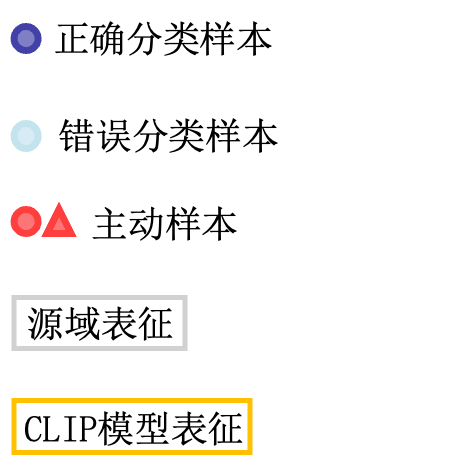
\includegraphics[width=0.23 \linewidth]{figures/chap4/indicator.png}}
    \bicaption[fig:points]{}{目标样本点在表征空间中的 t-SNE 可视化}{Fig.}{t-SNE visualization of the target sample points in the representation spaces}
\end{figure}


表~\ref{tab:ablation_sampling}对比了不同主动样本选择策略在有/无ViL模型监督下的性能：（1）不使用ViL模型时，MH Points在源模型假设空间下表现最优；（2）引入ViL模型后，仅依赖不确定性或多样性的策略（如ELPT、MH点集）甚至低于随机采样，而Core-Set和本章提出的DFSelector组合高于其他策略。这表明在多模型协作框架下，样本选择需同时兼顾双假设空间的几何覆盖与边界信息。
图~\ref{fig:points}给出了Office-Home 数据集 $C\xrightarrow{}P$ 任务上，不同采样策略下主动样本在源模型特征空间中的t-SNE分布~\cite{van2008visualizing}。可见ELPT样本集中于决策边界附近但多样性不足，Core-Set样本分布均匀但偏向类内中心，MH Points同时兼顾边界性与多样性。本章的DFSelector通过加权组合$\mathcal{T}_{MH}$（关注边界）与$\mathcal{T}_{CO}$（关注$\mathcal{Z}$空间覆盖），实现了双假设空间下的最优样本分布。


% \begin{figure}[!htbp]
%     \centering
%     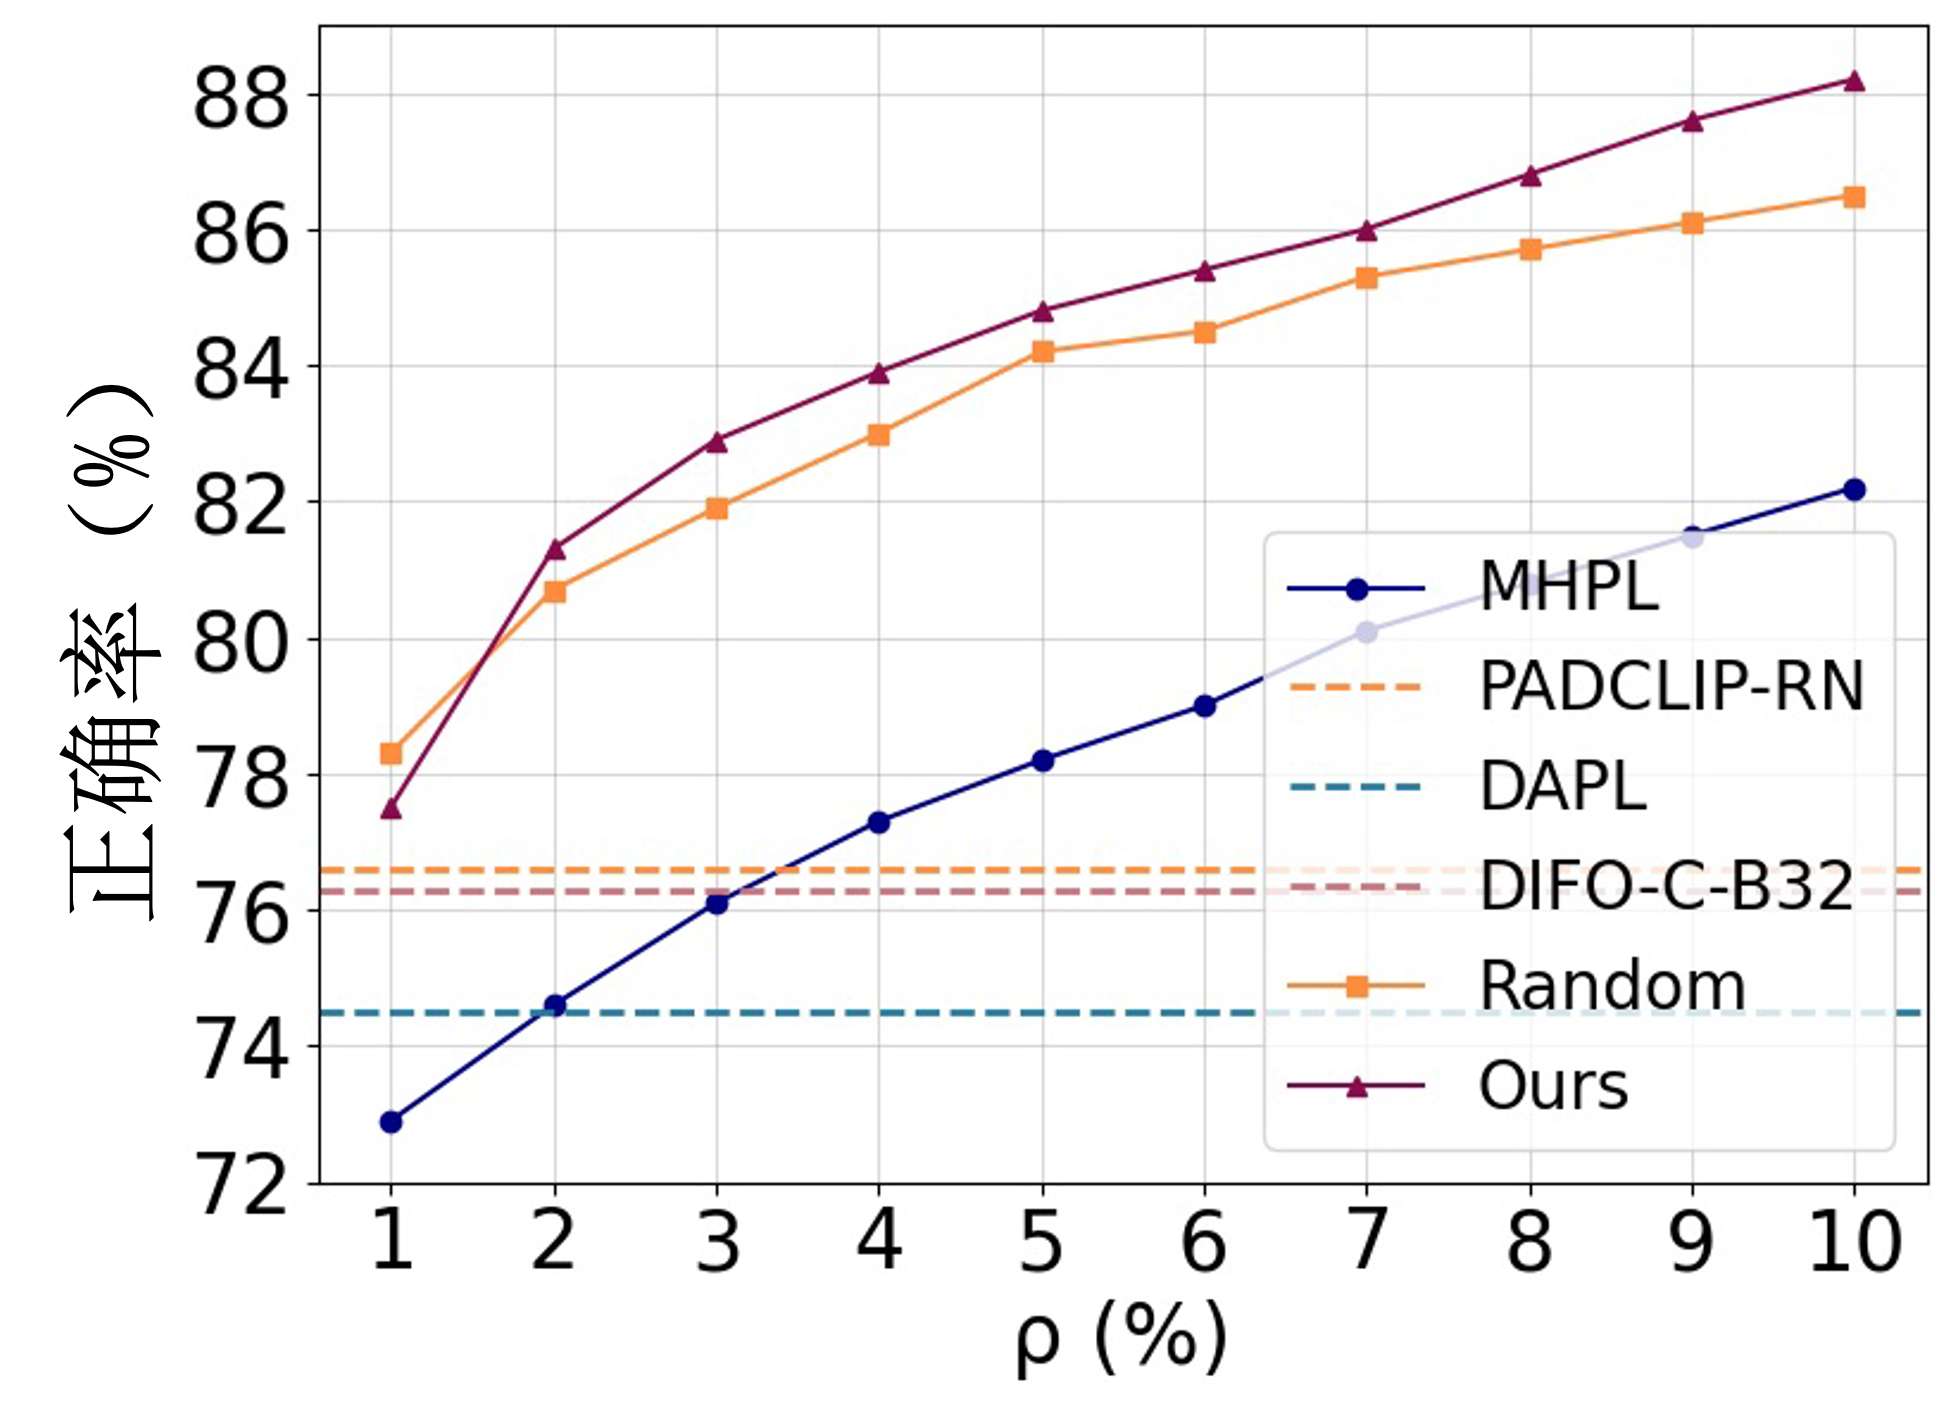
\includegraphics[width=0.62\textwidth]{figures/chap4/abl_active_ratio_uda.png}
%     \bicaption[fig:budget_compare]{}{不同标注预算下方法性能对比}{Fig.}{Performance under different labeling budgets}
% \end{figure}

% \begin{figure}[!htbp]
%     \centering
%     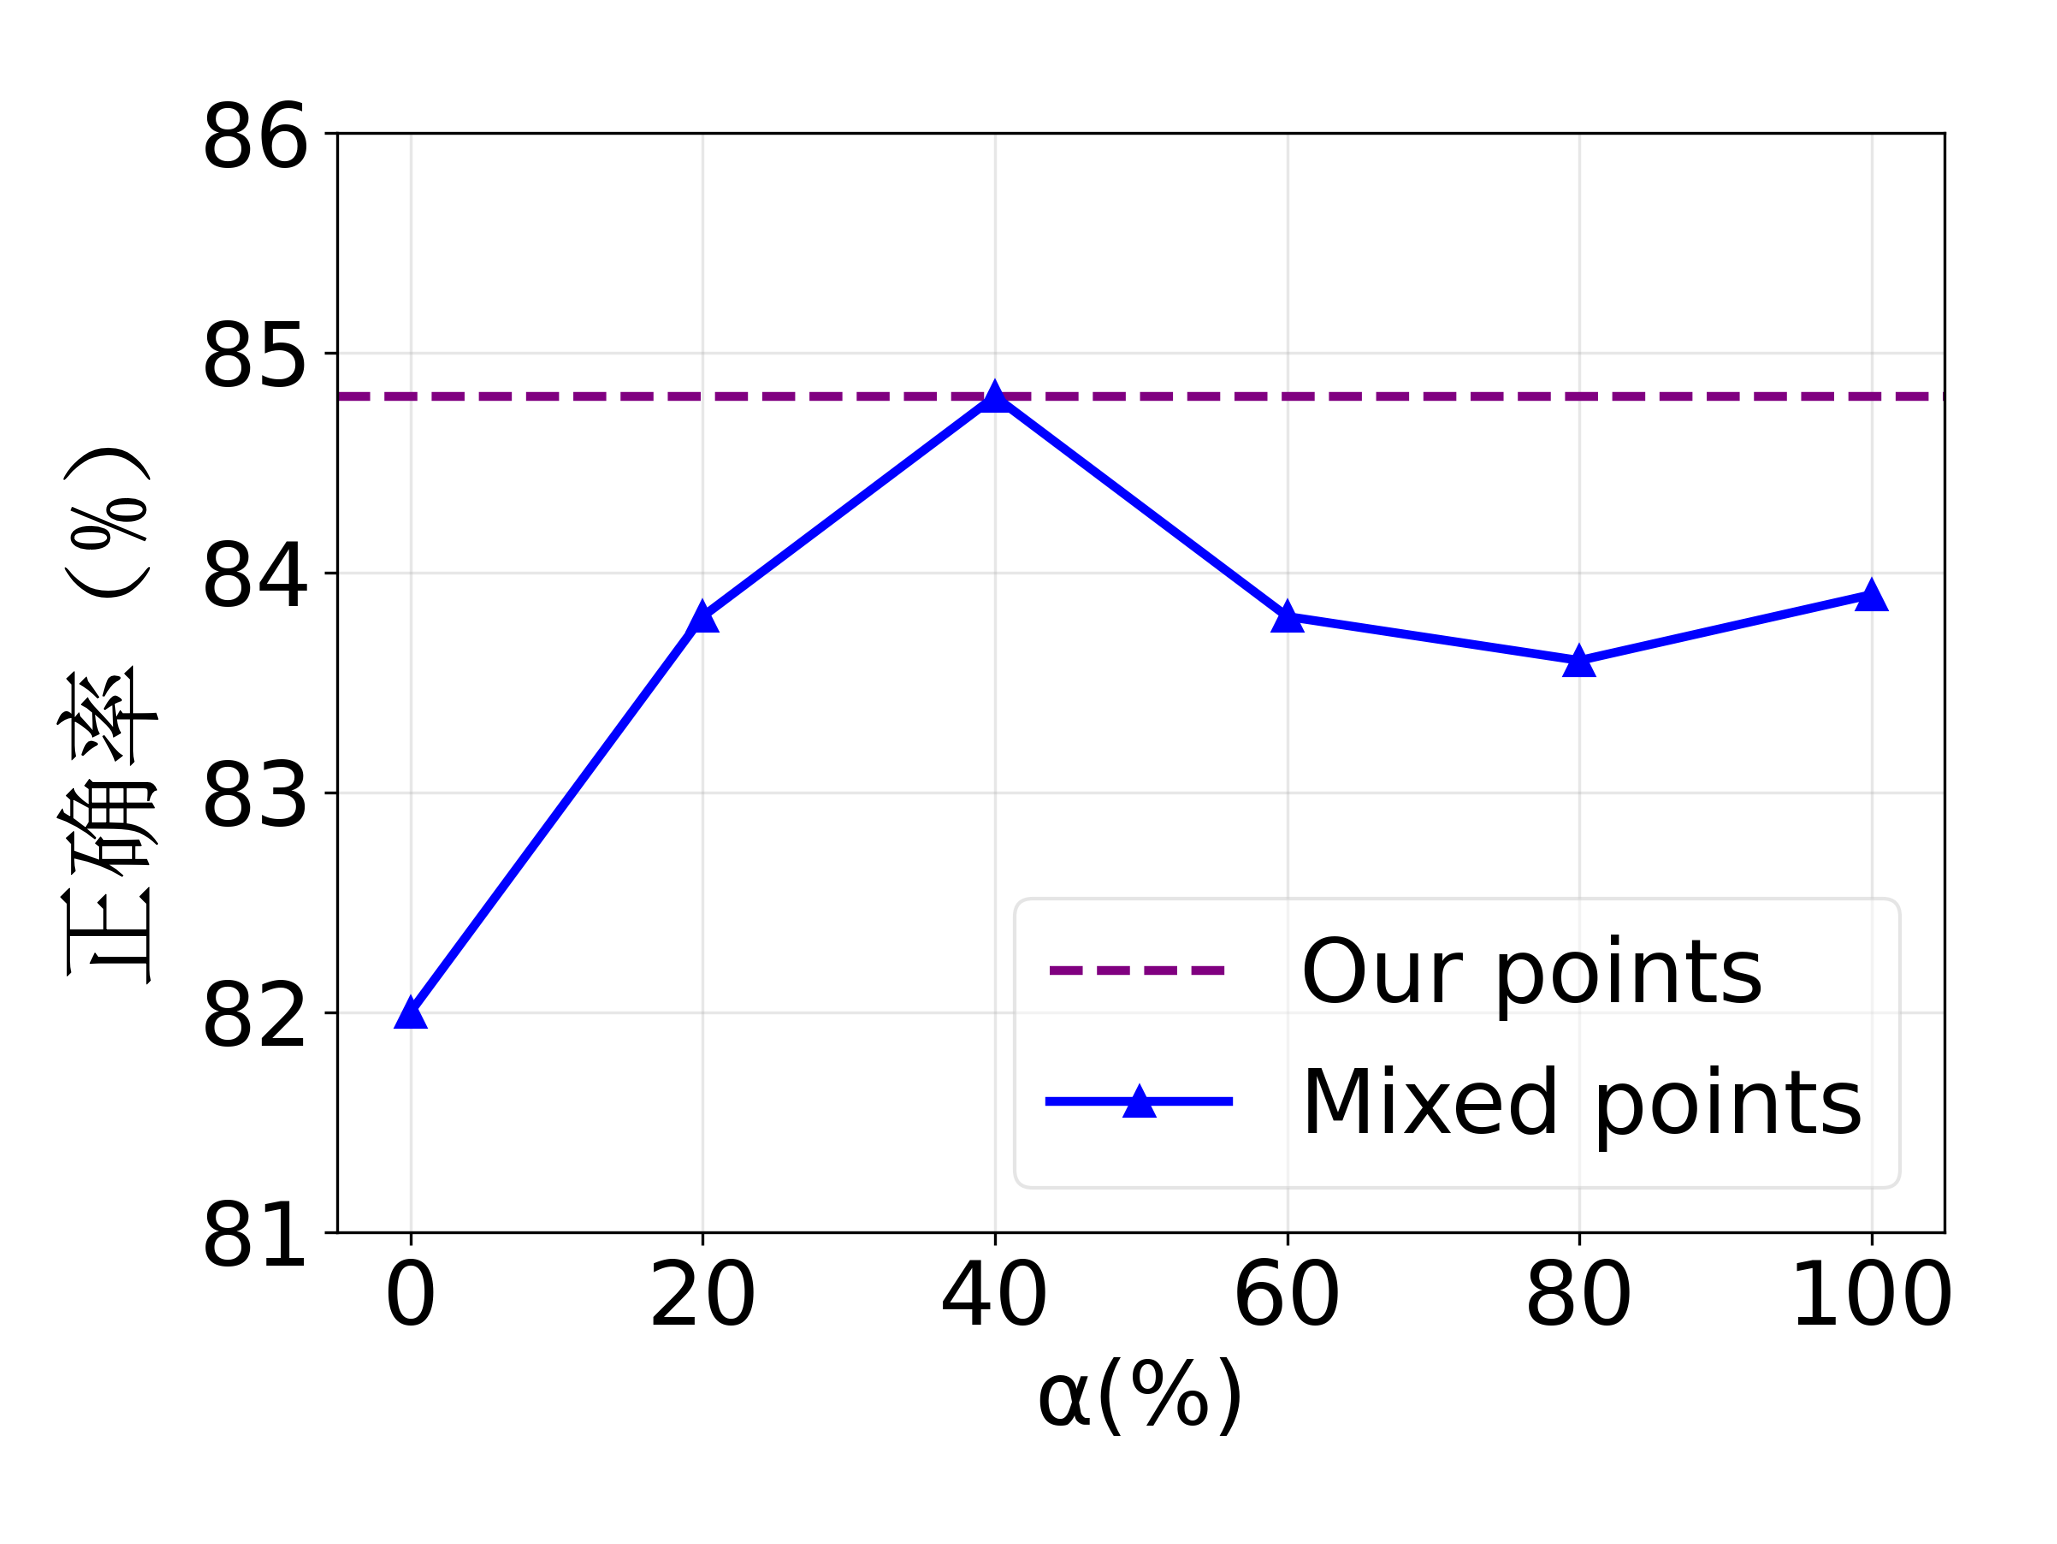
\includegraphics[width=0.5\textwidth]{figures/chap4/mixed_model_alpha_re.png}
%     \bicaption[fig:alpha_analysis]{}{样本选择比例$\alpha$对性能的影响}{Fig.}{Impact of balance ratio $\alpha$}
% \end{figure}

\begin{figure}[!htbp]
    \centering
    \setlength{\tabcolsep}{0pt}
    \subfigure[]{
    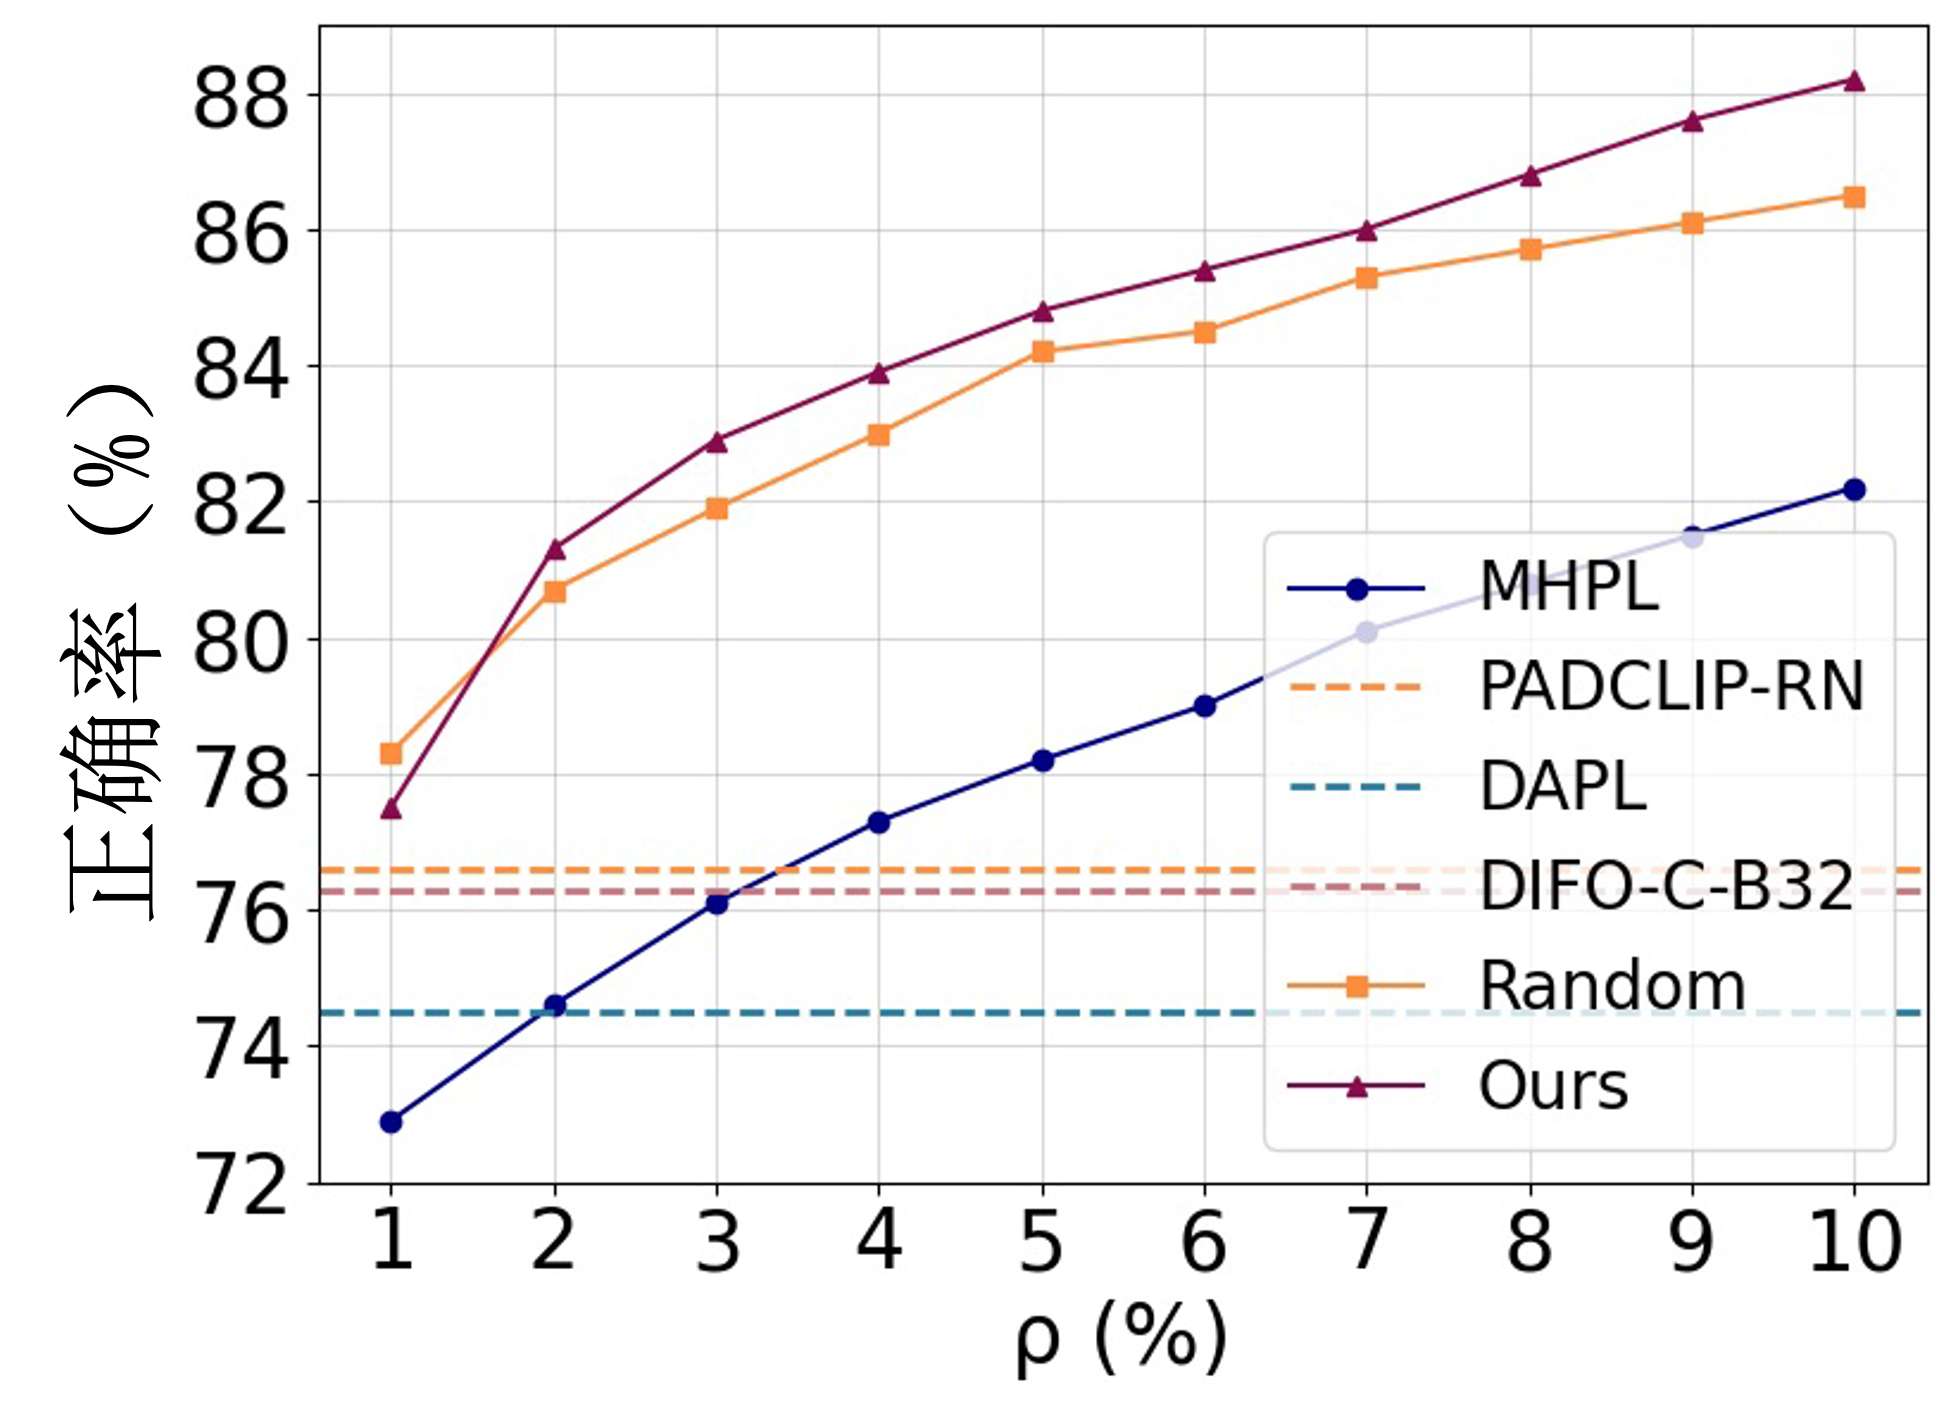
\includegraphics[width=0.3\linewidth]{figures/chap4/abl_active_ratio_uda.png}
        \label{fig:budget_compare}
    }
    \subfigure[]{
    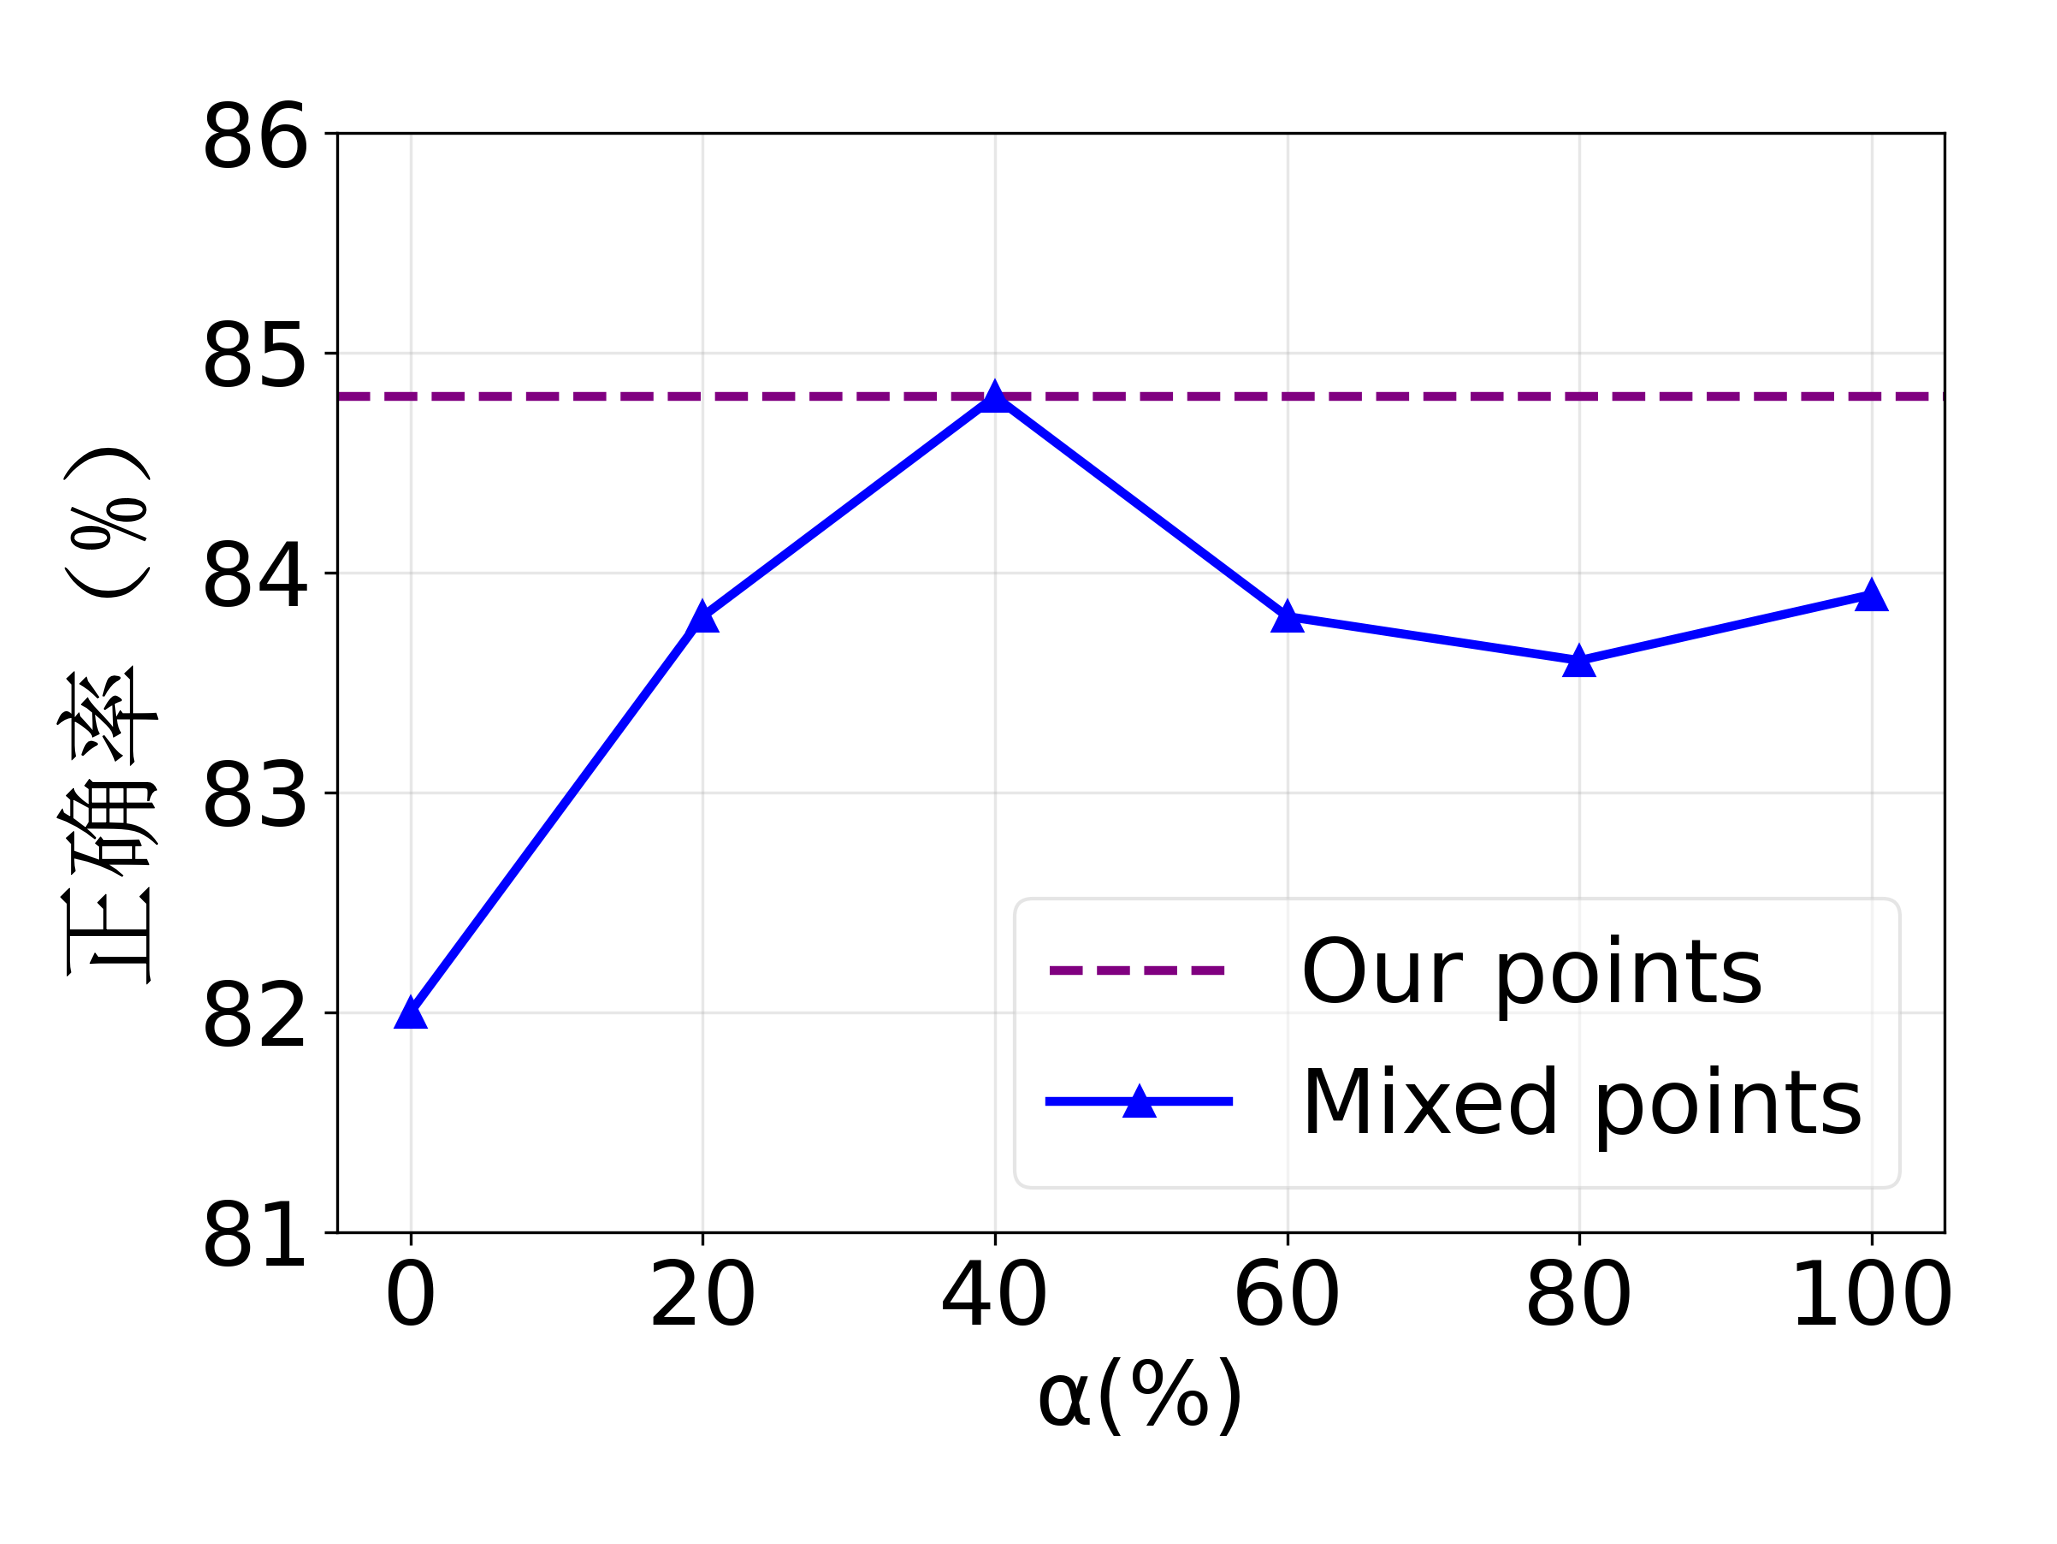
\includegraphics[width=0.3\linewidth]{figures/chap4/mixed_model_alpha_re.png}
        \label{fig:sub_alpha_analysis}
    }
    \subfigure[]{
    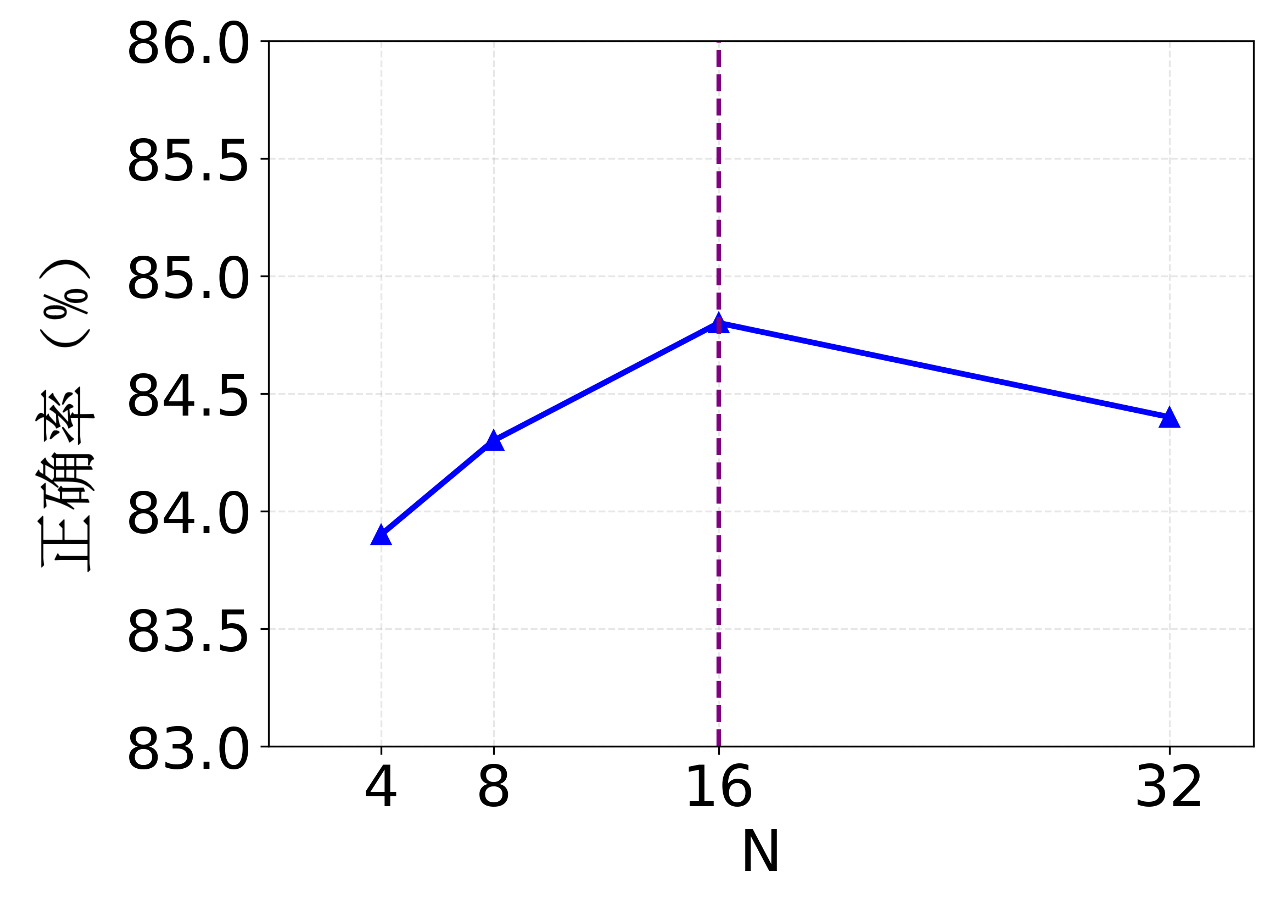
\includegraphics[width=0.3\linewidth]{figures/chap4/accuracy_curve.png}
        \label{fig:abl_n}
    }
\bicaption[fig:alpha_analysis]{}{Office-Home数据集上的参数消融对比}{Fig.}{Parameter ablations on the Office-Home dataset}
\end{figure}


图~\ref{fig:alpha_analysis}包含三组实验，其中子图（a）所示的标注预算对比已在主实验部分分析，此处进一步考察加权比例$\alpha$与目标样本选择大小$N$对性能的影响。
子图（b）给出$\mathcal{T}_{CO}$与$\mathcal{T}_{MH}$加权比例$\alpha$对性能的影响。性能在$\alpha=0.4$处达到峰值，与主实验所报告的性能水平一致；越过该最优点后性能下降并最终趋于平台。该结果印证了$\mathcal{T}_{CO}$与$\mathcal{T}_{MH}$两类样本贡献之间的权衡关系：$\alpha$过大时标注集偏向$\mathcal{Z}$空间的几何覆盖而缺乏$\mathcal{X}$空间的边界信息，过小则偏向边界信息捕获而忽略ViL模型的适配需求，因此中间取值构成最优配置。
子图（c）分析目标样本选择大小$N$的影响，即式\eqref{eq:topX}所涉$\mathcal{X}_{top}$集合中每类保留的高置信样本数。当$N$从4增至32时性能先升后降，在$N=16$处取得峰值。过小的$N$将蒸馏目标限制在极少数高置信样本上，削弱了知识传递信号；过大的$N$则引入噪声预测，破坏ViL模型的对齐质量。据此本文将$N=16$设为全部实验的默认取值。

图~\ref{fig:lambda_sensitivity}给出了知识保持正则系数$\lambda$的影响：闭集场景下$\lambda=1$最优，开放集场景下$\lambda=8$最优。这是因为开放集任务中保留ViL模型的泛化能力对未知类别检测尤为关键。图~\ref{fig:beta_sensitivity}给出了样本权重$\beta_q$与$\beta$的影响：较高的$\beta_q$有助于突出真实标注样本的贡献，而$\beta$在0.3附近表现最佳，过大或过小均会因过度利用或抑制伪标签而损害性能。


\begin{figure}[!htbp]
    \centering
    \subfigure[闭集]{
    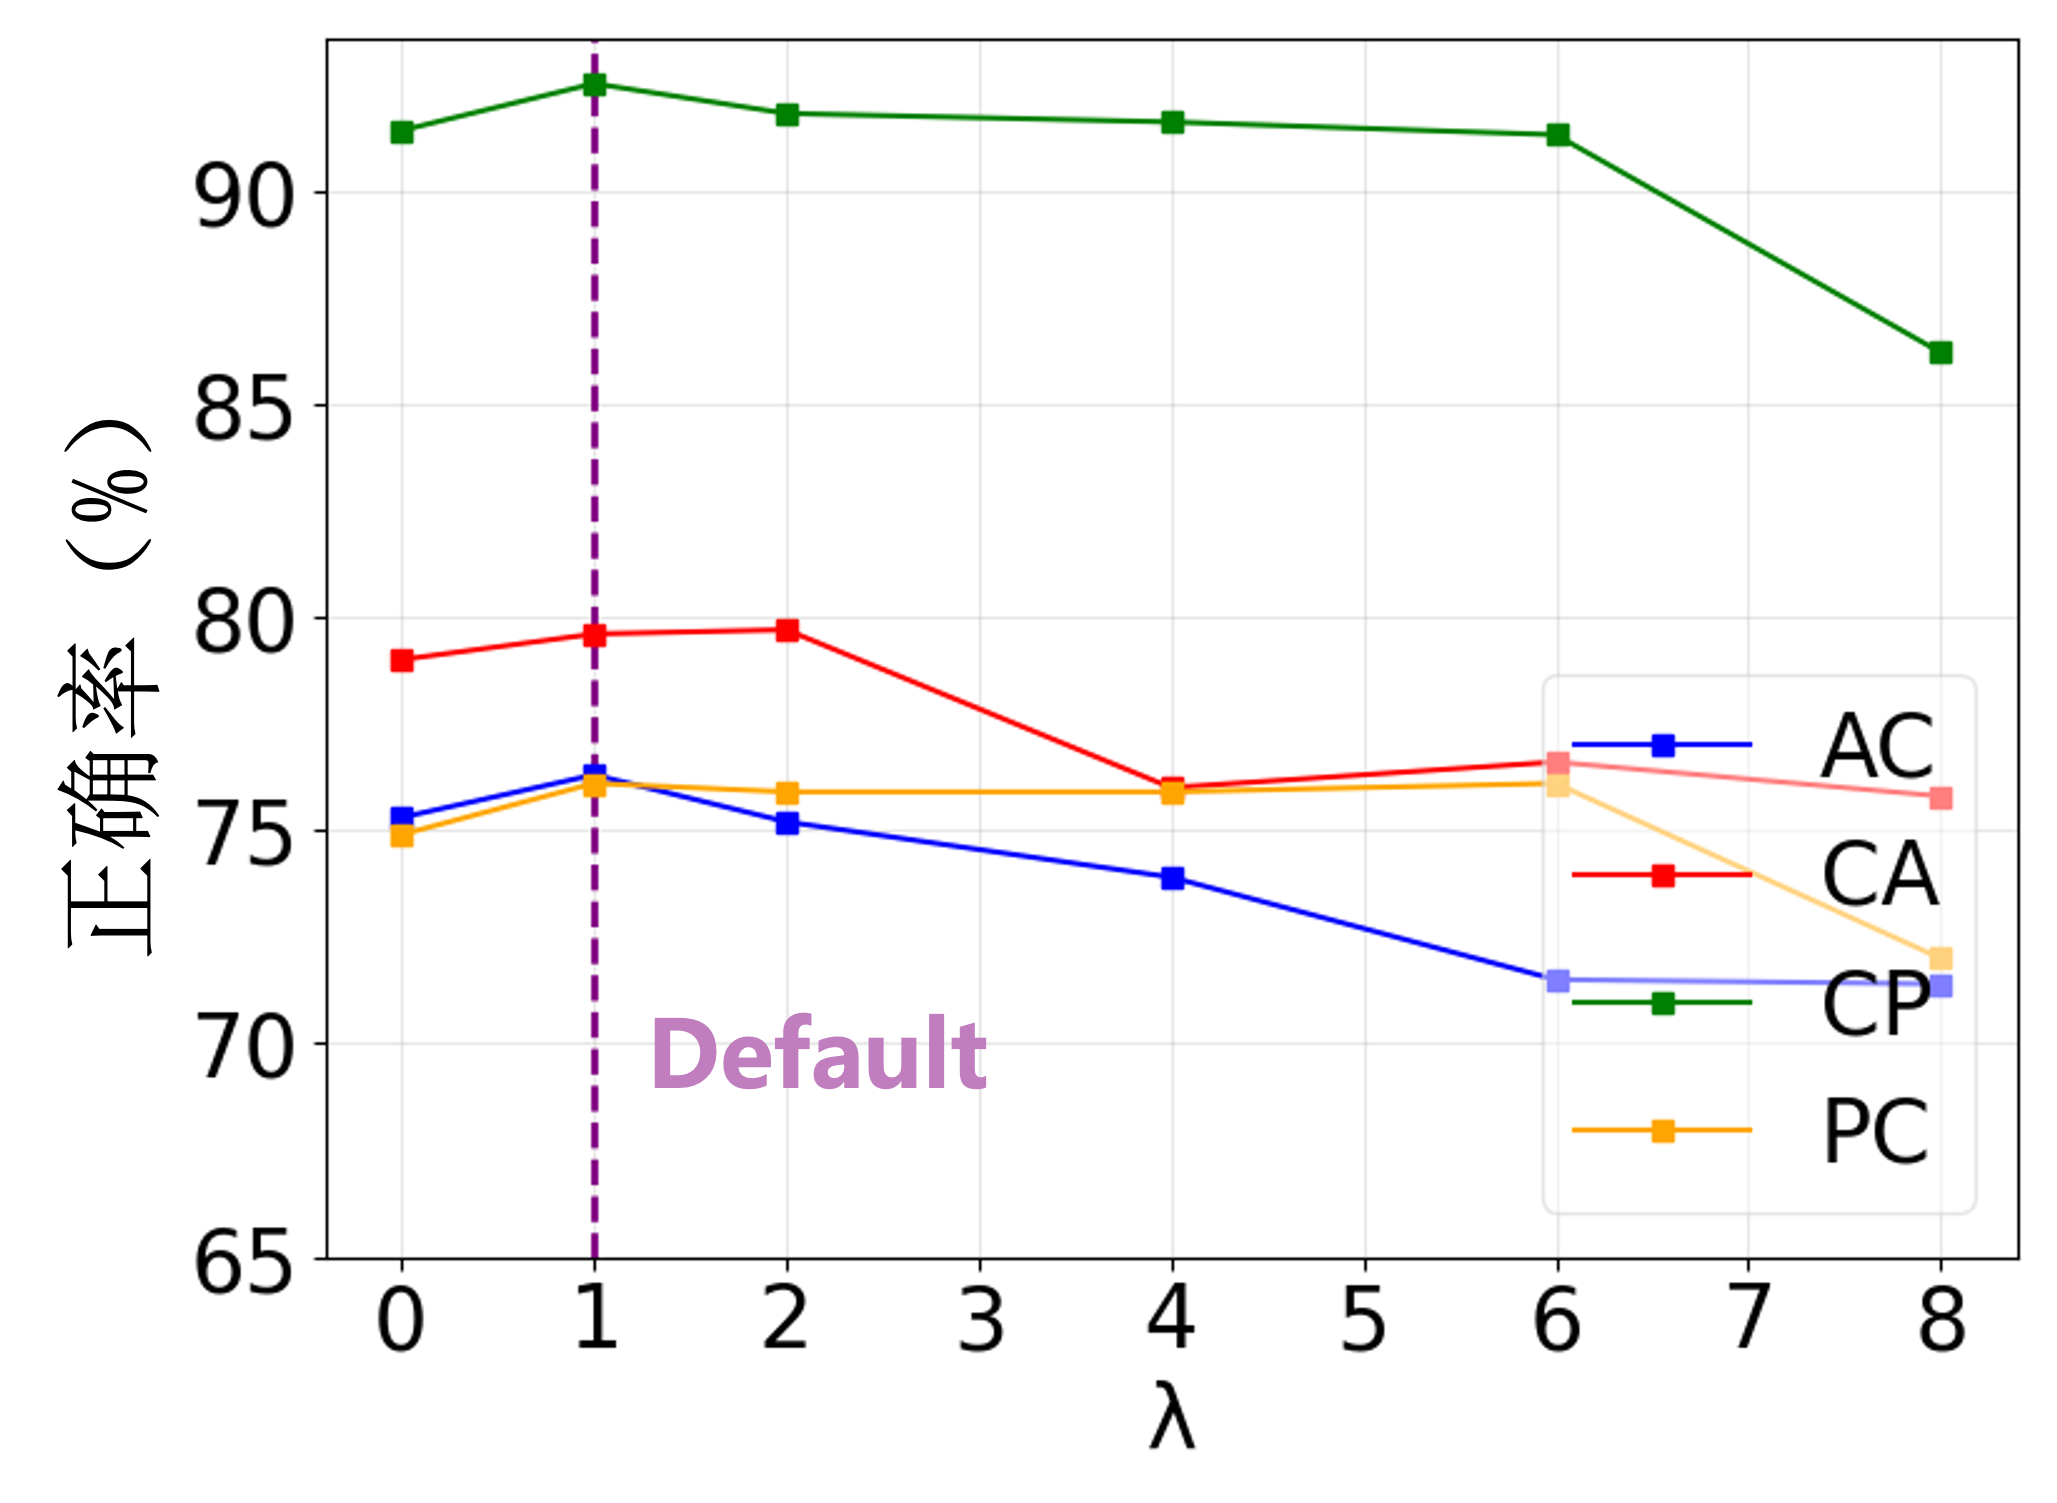
\includegraphics[width=0.35\linewidth]{figures/chap4/uda_lambda.png}}   
    \subfigure[开集]{
    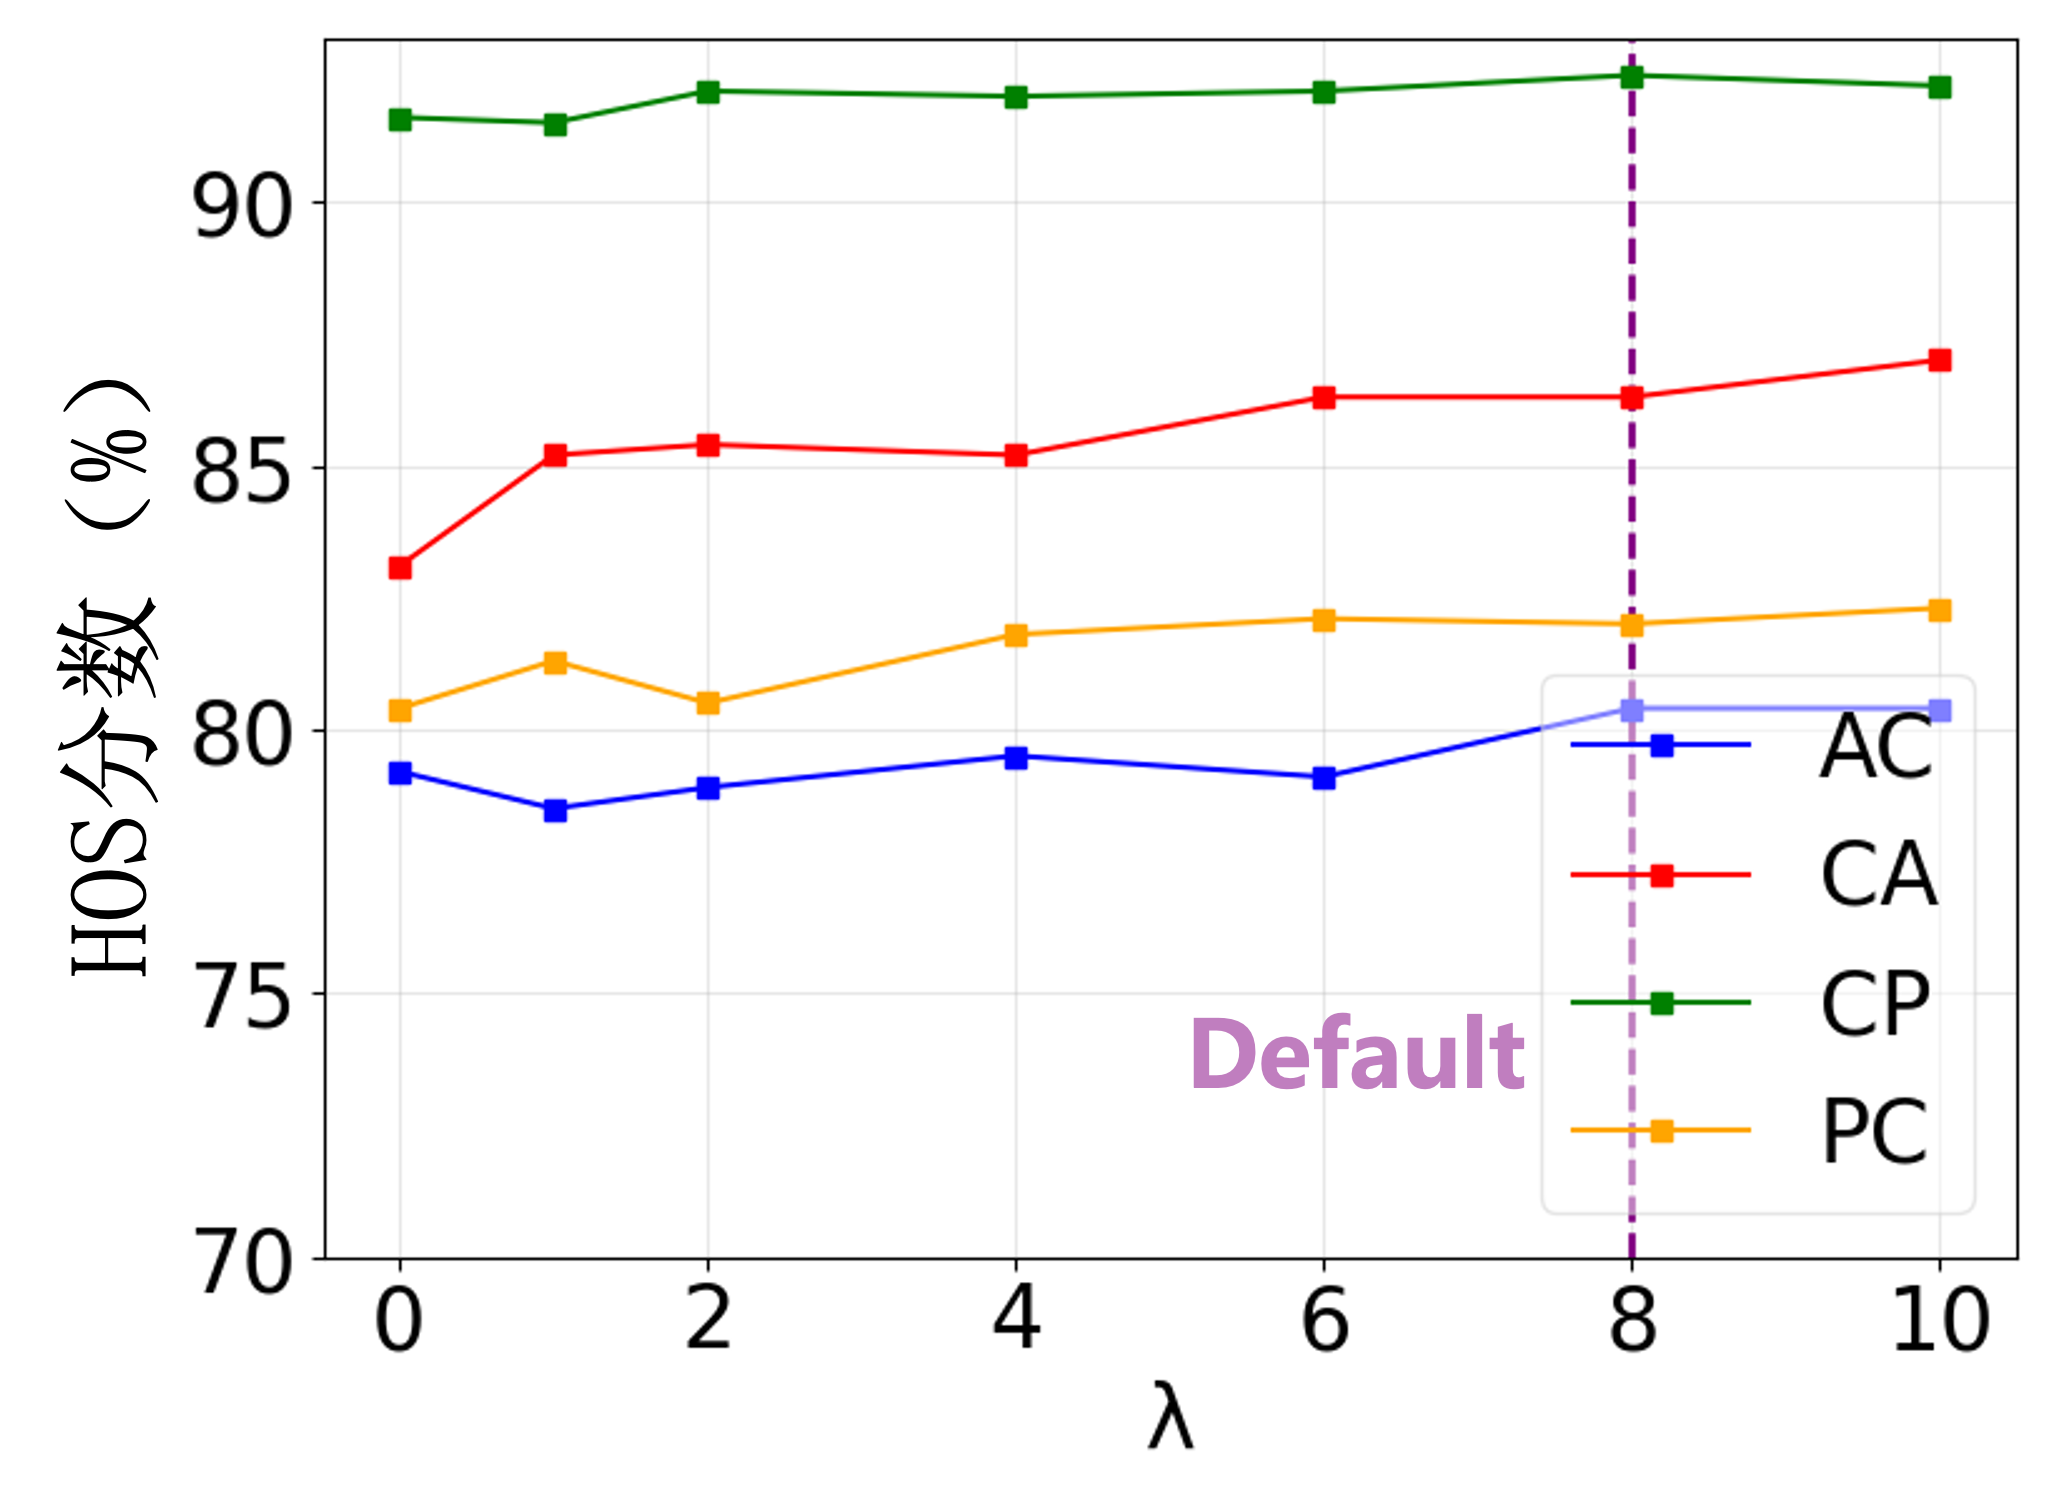
\includegraphics[width=0.35\linewidth]{figures/chap4/oda_lambda.png}}
    \bicaption[fig:lambda_sensitivity]{}{正则系数$\lambda$消融}{Fig.}{Impact of regularization weight $\lambda$}
    \label{fig:lambda}
\end{figure}

\begin{figure}[!htbp]
    \centering
    \subfigure[]{
    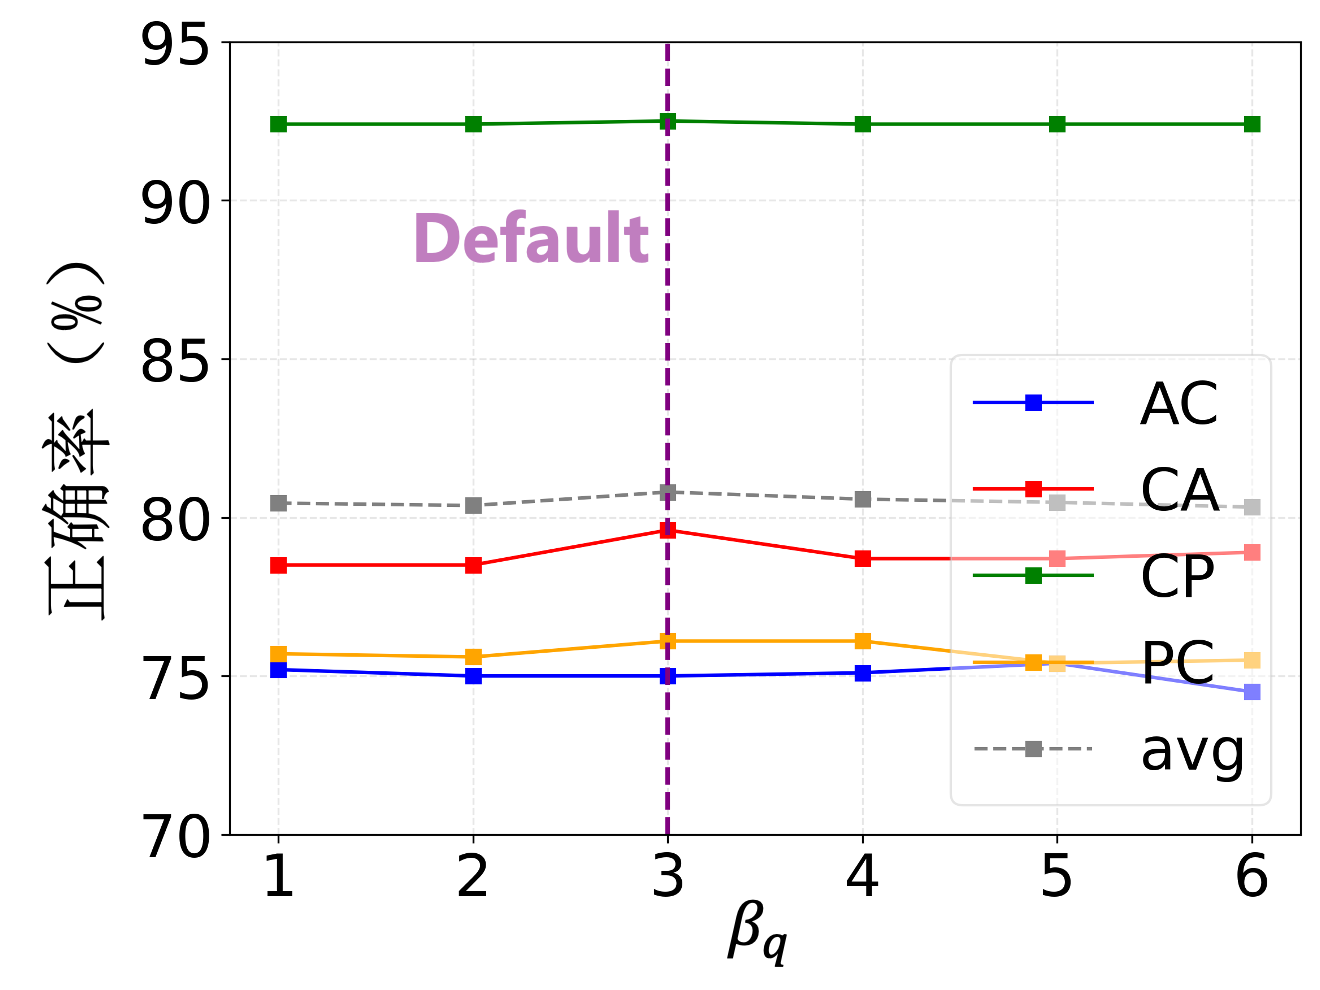
\includegraphics[width=0.35\linewidth]{figures/chap4/abl_betaq.png}}   
    \subfigure[]{
    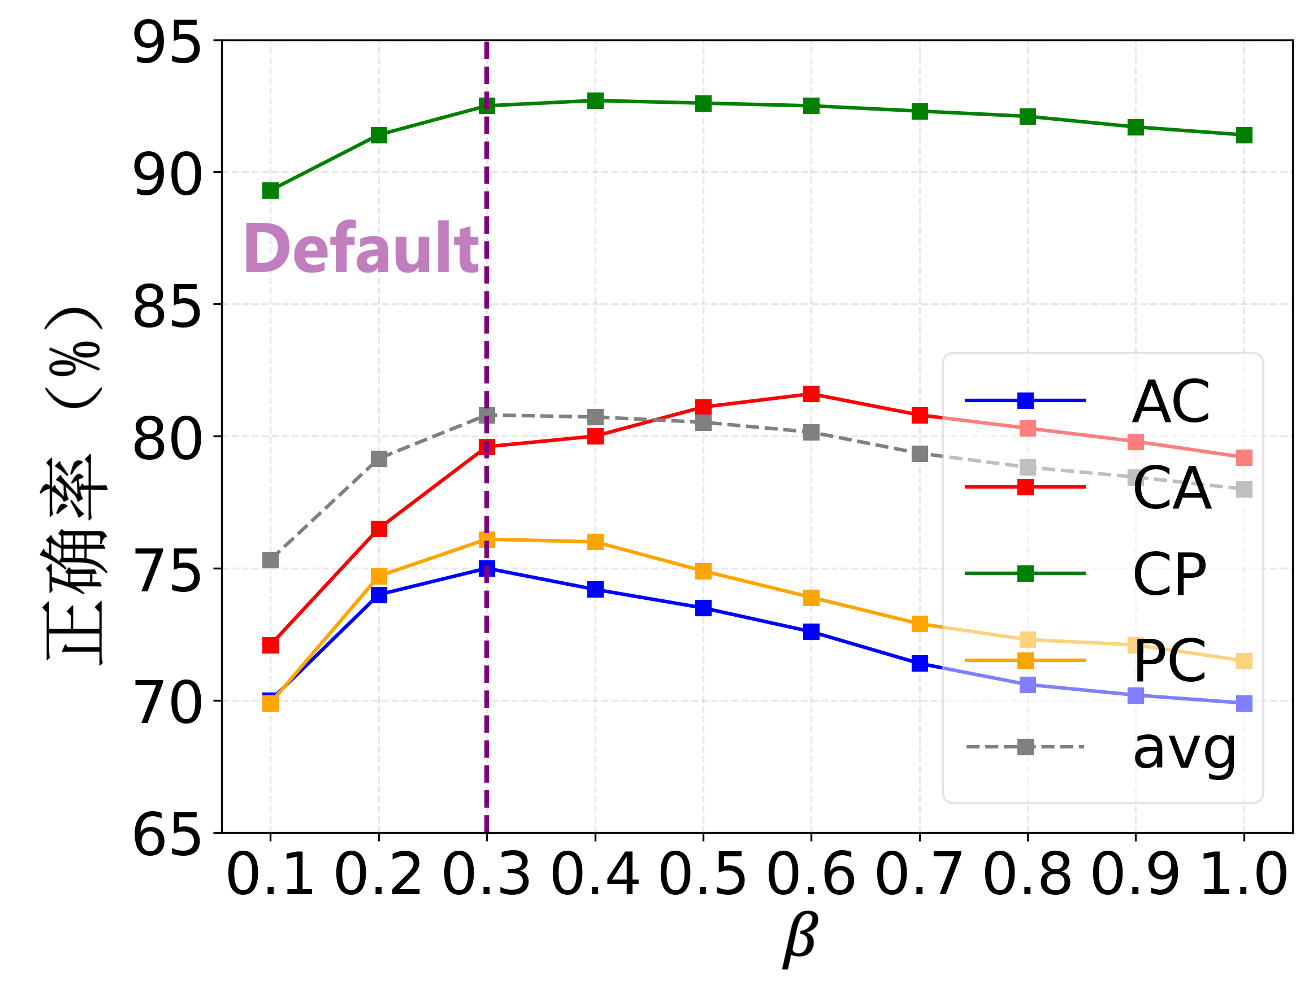
\includegraphics[width=0.35\linewidth]{figures/chap4/abl_beta.png}}
    \bicaption[fig:beta_sensitivity]{}{样本权重$\beta_q$与$\beta$消融}{Fig.}{Ablations of sample weights $\beta_q$ and $\beta$}
    % \caption{Impact of sample weights $\beta_q$ and $\beta$ on the transfer tasks in Office-Home. We report both individual task-wise performance and their average (line 'avg'). The purple dashed line indicates the \textit{Default} setting.}
    \label{fig:beta}
\end{figure}


表~\ref{tab:clip_evolution}给出了ViL模型（CLIP）在适应过程中的性能演化。结果显示，CLIP在APT阶段（CUS-C-B32）已获得显著增益，表明主动标注样本对CLIP的类别prompt适配极具价值；进一步经ADL蒸馏后（DAMF-ViL），CLIP性能继续提升。然而DAMF-ViL仍低于完整DAMF，说明ViL模型与目标模型的协作能够实现1+1>2的协同效应。

\begin{table}[!htbp]
    \bicaption[tab:clip_evolution]{}{适应过程中CLIP的准确率演化}{Table}{CLIP accuracy evolution throughout adaptation}
    \vspace{0.5em}\centering\wuhao
    % \resizebox{.9\textwidth}{!}{
    \begin{tabular}{lcccc}
    \toprule
    方法 & Office-Home & VisDA-C & Office & miniDomainNet \\
    \midrule
    ZS-C-B32 & 72.2 & 87.2 & 79.5 & 80.0 \\
    CUS-C-B32 (使用APT后) & 80.0 (+7.8) & 90.2 (+3.0) & 80.9 (+1.4) & 83.5 (+3.5) \\
    DAMF-ViL (使用ADL后)  & 81.7 (+1.7) & 92.1 (+1.9) & 88.8 (+7.9) & 84.0 (+0.5) \\
    \bottomrule
    \end{tabular}  
    % }
\end{table}

\begin{figure}[!htbp]
    \centering
    \subfigure[源域模型(63.3\%)]{\includegraphics[width=0.23\linewidth]{papers/DAMF/tsne_source.pdf}
    \label{fig:res_tsne_a}
    }
\vrule
    \subfigure[ELPT(80.7\%)]{\includegraphics[width=0.23\linewidth]{papers/DAMF/tsne_ELPT.pdf}
    \label{fig:res_tsne_elpt}}
    \subfigure[MHPL(82.6\%)]{\includegraphics[width=0.23\linewidth]{papers/DAMF/tsne_MHPL.pdf}
    \label{fig:res_tsne_mhpl}}
    \subfigure[本章(86.6\%)]{\includegraphics[width=0.23\linewidth]{papers/DAMF/tsne_mine.pdf}
    \label{fig:res_tsne_mine}}
    \bicaption[fig:tsne_features]{}{不同采样策略下主动样本分布的t-SNE可视化}{Fig.}{t-SNE visualization of active samples under different strategies}
\end{figure}

图~\ref{fig:tsne_features}给出了Office数据集W$\rightarrow$A任务上目标特征在适应前后的t-SNE分布。适应前特征分布较为分散，类间边界模糊；适应后DAMF的特征聚类最为紧凑，且误分类样本（灰色三角形）显著少于ELPT和MHPL，验证了本章方法在域适应效果上的优越性。

表~\ref{tab:cost}对比了有无ViL模型情况下的训练与推理开销。DAMF在训练阶段仅增加0.002M可训练参数（prompt参数）和0.48 GB GPU显存（+8.8\%），额外计算量可忽略。闭集推理阶段ViL模型被完全丢弃，对推理速度无影响；开放集推理阶段虽然需要额外调用ViL模型进行未知类别检测，但相比基于聚类的开放集方法（如MHPL-O的2-类k-means聚类），DAMF无需任何预处理时间，反而实现了更高的推理吞吐（339.74 FPS vs 212.68 FPS）。

\begin{table}[!htbp]
    \bicaption[tab:cost]{}{训练与推理开销对比}{Table}{Training and inference cost comparison}
    \vspace{0.5em}\centering\wuhao
    \begin{tabular}{cccc}
    \toprule
    \multirow{2}{*}{ViL} & \multicolumn{2}{c}{训练} & 推理（开放集） \\
    \cline{2-4}
    & 可训练参数 [M] & 峰值显存 [GB] & FPS \\
    \midrule
    $\times$ & 24.041 & 5.43 & 212.68$^\dagger$ \\
    \checkmark (本章) & 24.043 (+0.002) & 5.91 (+0.48) & 339.74 \\
    \bottomrule
    \end{tabular}
\end{table}

\FloatBarrier
\section{本章小结}

本章围绕视觉—语言基础模型与稀缺主动标注难以有效协同的问题，沿样本筛选与跨模型协同两个角度协同推进。在样本筛选层面，借助双假设空间下的样本覆盖度量选择最具信息量的目标样本，突破简单组合框架下的性能瓶颈；在跨模型协同层面，借助任务感知的提示激活与双向知识互补机制实现视觉—语言模型与目标模型之间的稳定融合，避免视觉—语言模型丧失泛化能力。理论层面，本章推导了 SFADA 协作风险上界，明确了双假设空间下的样本覆盖、视觉—语言模型的目标域风险与跨模型对齐损失三个关键因素的协同优化目标。实验在闭集与开放集两种设定下均取得当前最优性能，验证了所提框架的有效性与工程实用性，并为下一章在开放类设定下将视觉—语言模型的开放语义与分割基础模型的空间定位能力进一步深度融合奠定了双模型协同的框架基础。

% Local Variables:% Local Variables:
% TeX-master: "../thesis"
% TeX-engine: xetex
% End:
